\chapter{Attivazioni dei Modelli}

Nelle seguenti figure vengono mostrate le rappresentazioni PCA delle attivazioni estratte dai modelli dagl LLM. Le attivazioni sono state ottenute da tre tipi di layer: Attention, MLP e Hidden. In rosso sono indicate le istanze allucinatorie, mentre in blu quelle veritiere.
\newpage
\begin{figure}[H]
    \centering
    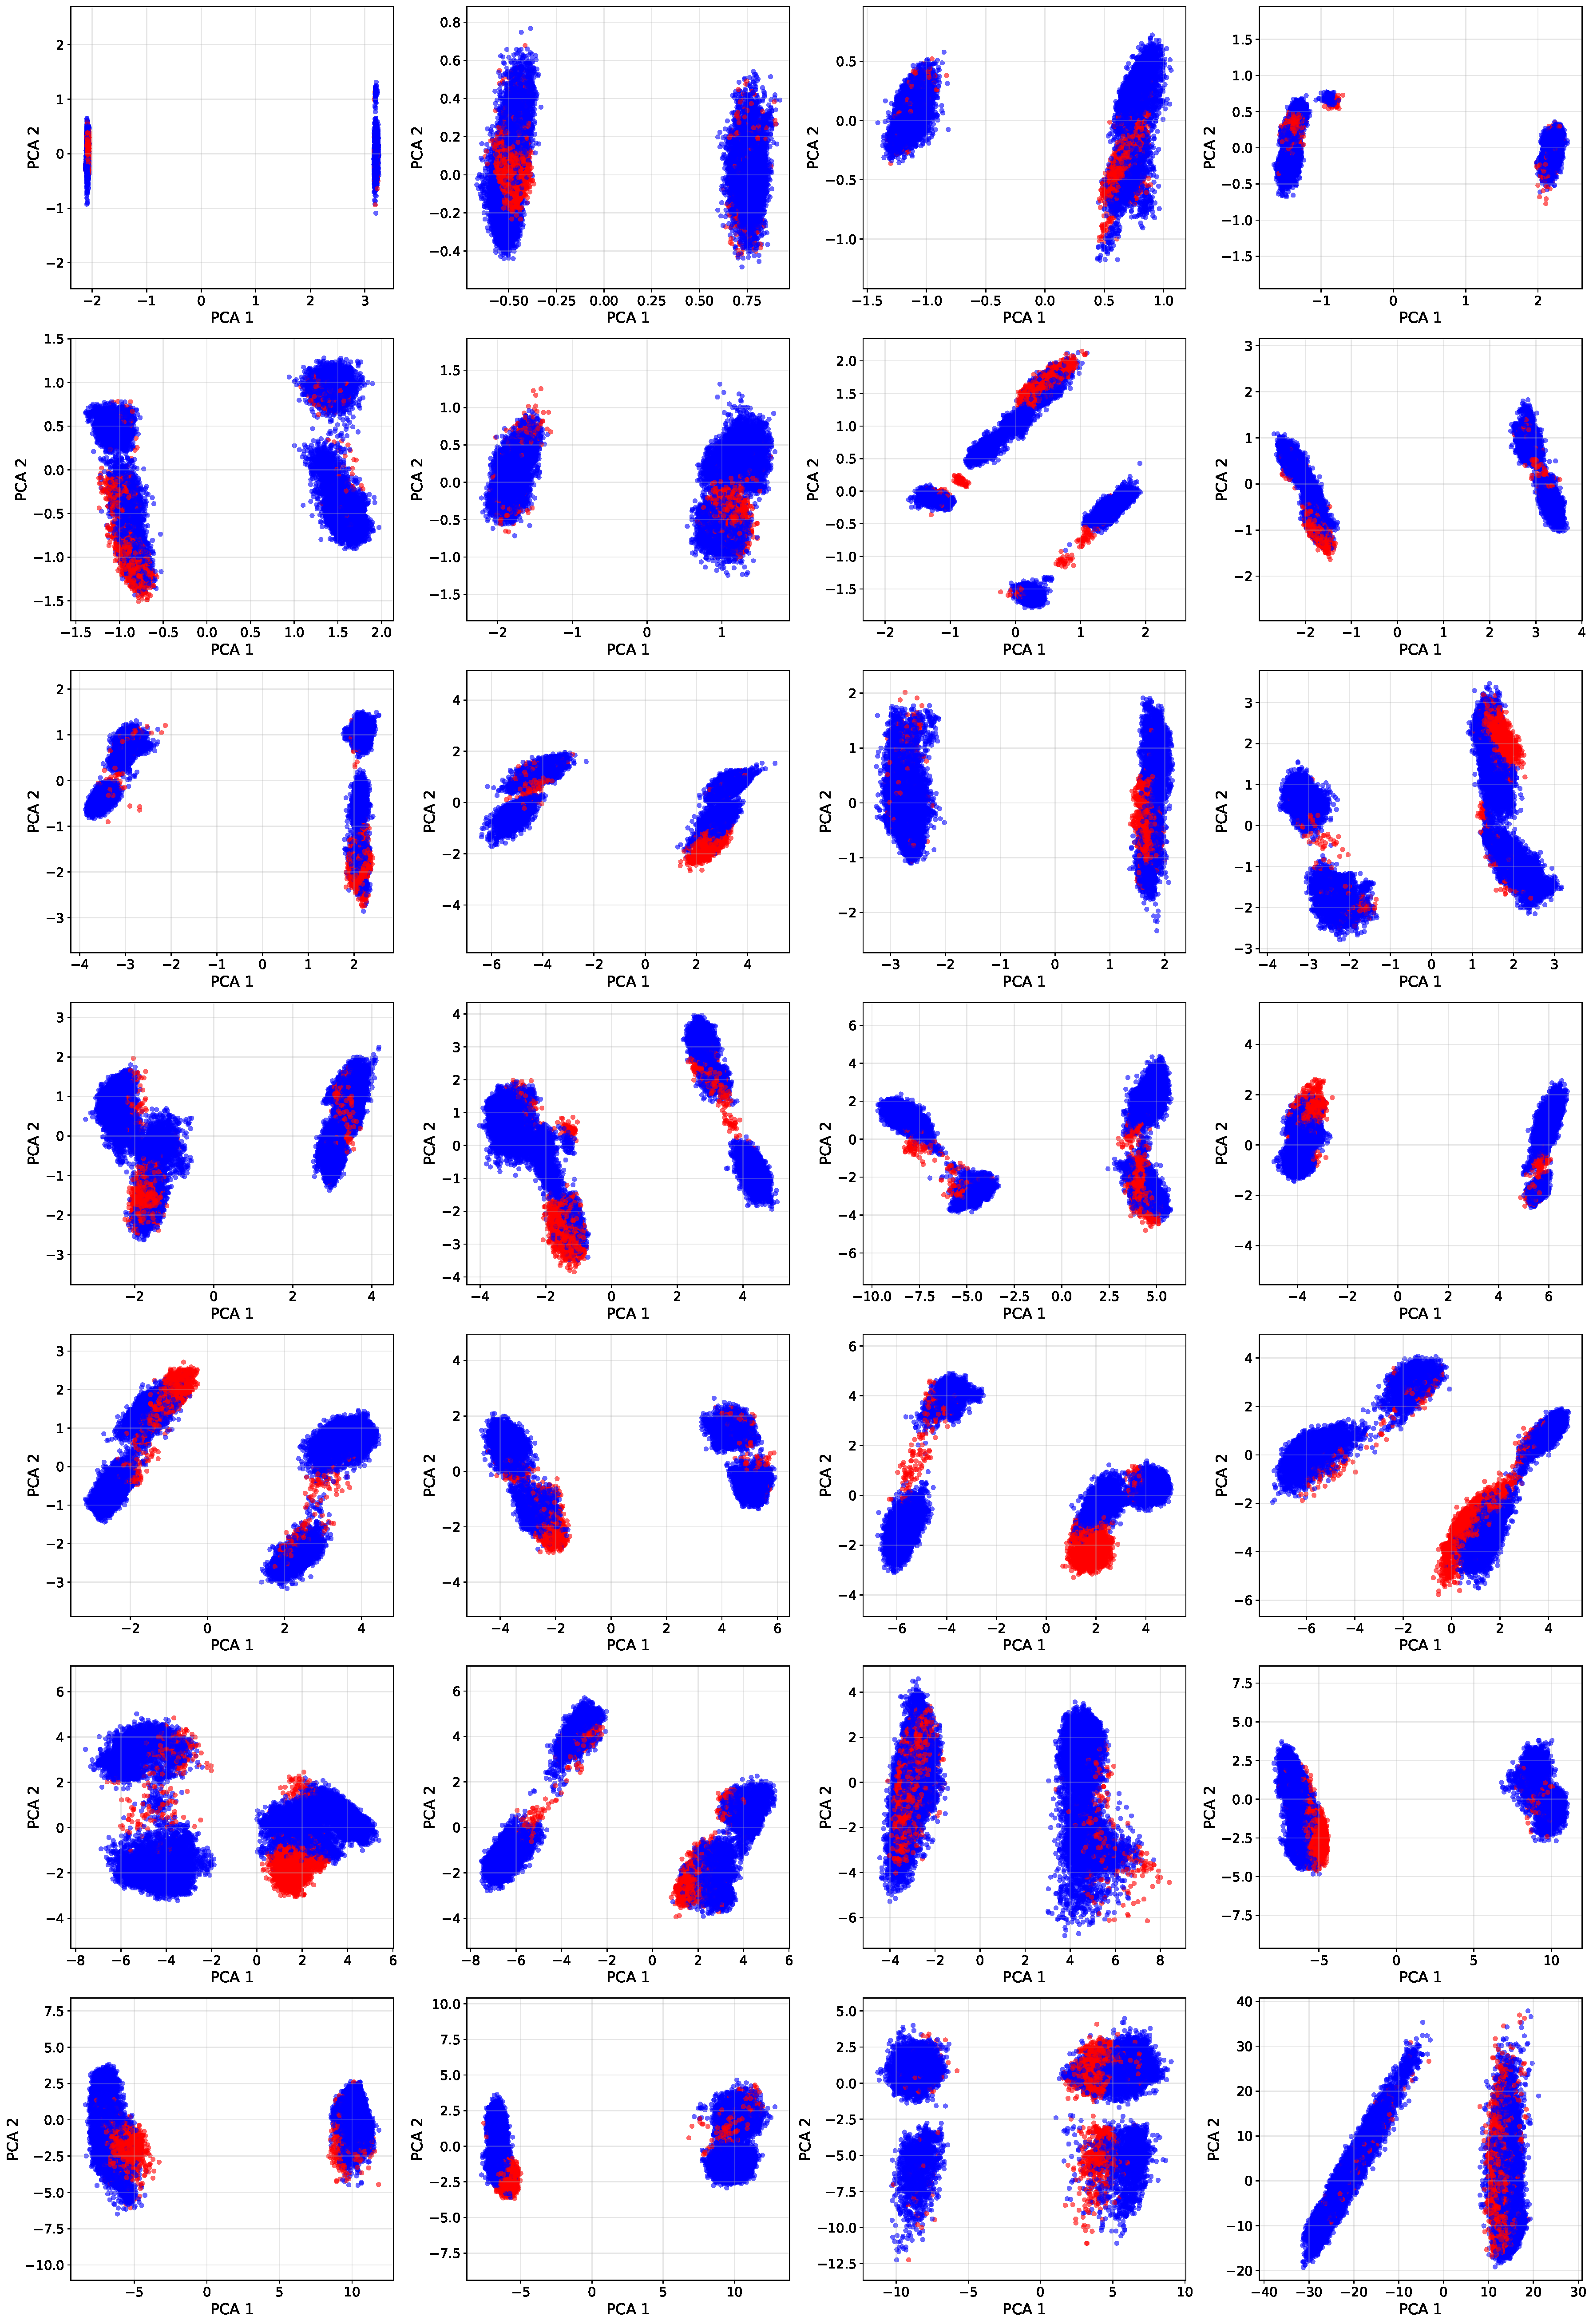
\includegraphics[width=\textwidth, height=1\textheight, keepaspectratio]{images/PCA_Plots/Qwen2.5-7B_belief_bank_facts_attn_activations_PCA_CLEAN.pdf}
    \caption{PCA delle attivazioni Attention del layer di Qwen2.5-7B per Belief Bank Facts}
    \label{fig:qwen-pca-attn-facts-full}
\end{figure}

\begin{figure}[H]
    \centering
    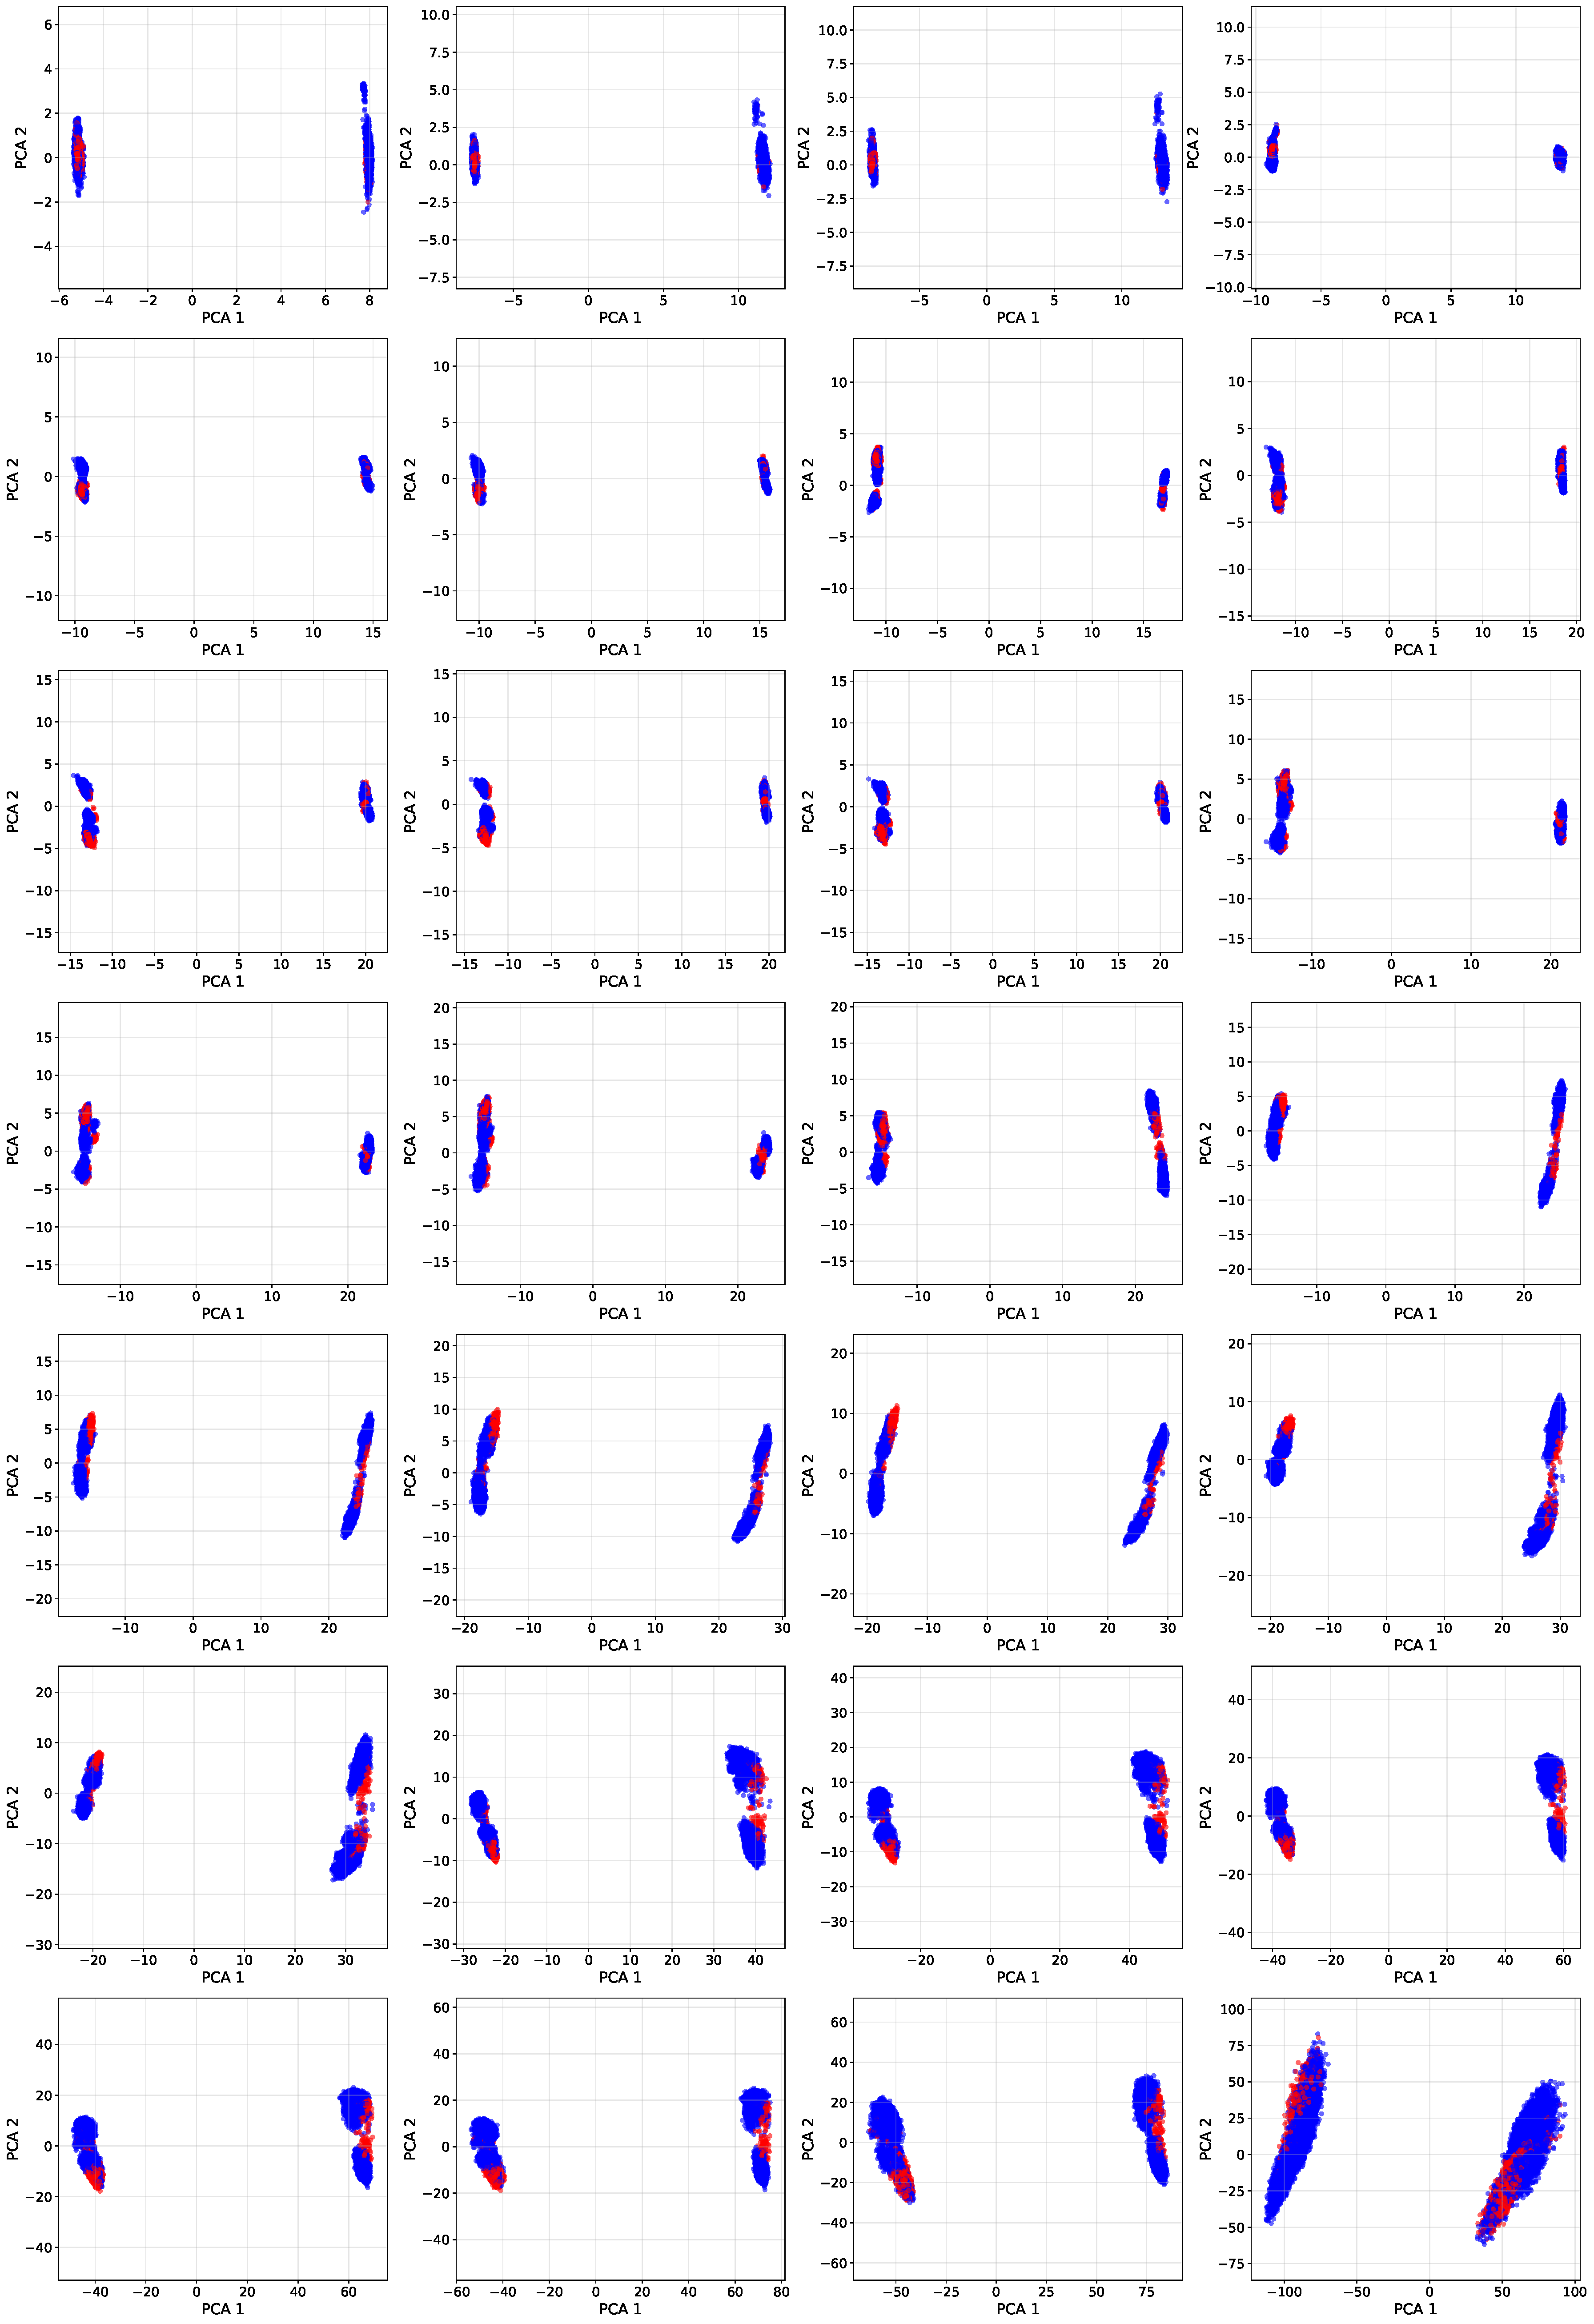
\includegraphics[width=\textwidth, height=1\textheight, keepaspectratio]{images/PCA_Plots/Qwen2.5-7B_belief_bank_facts_hidden_activations_PCA_CLEAN.pdf}
    \caption{PCA delle attivazioni Hidden del layer di Qwen2.5-7B per Belief Bank Facts}

    \label{fig:qwen-pca-hidden-facts-full}
\end{figure}

\begin{figure}[H]
    \centering
    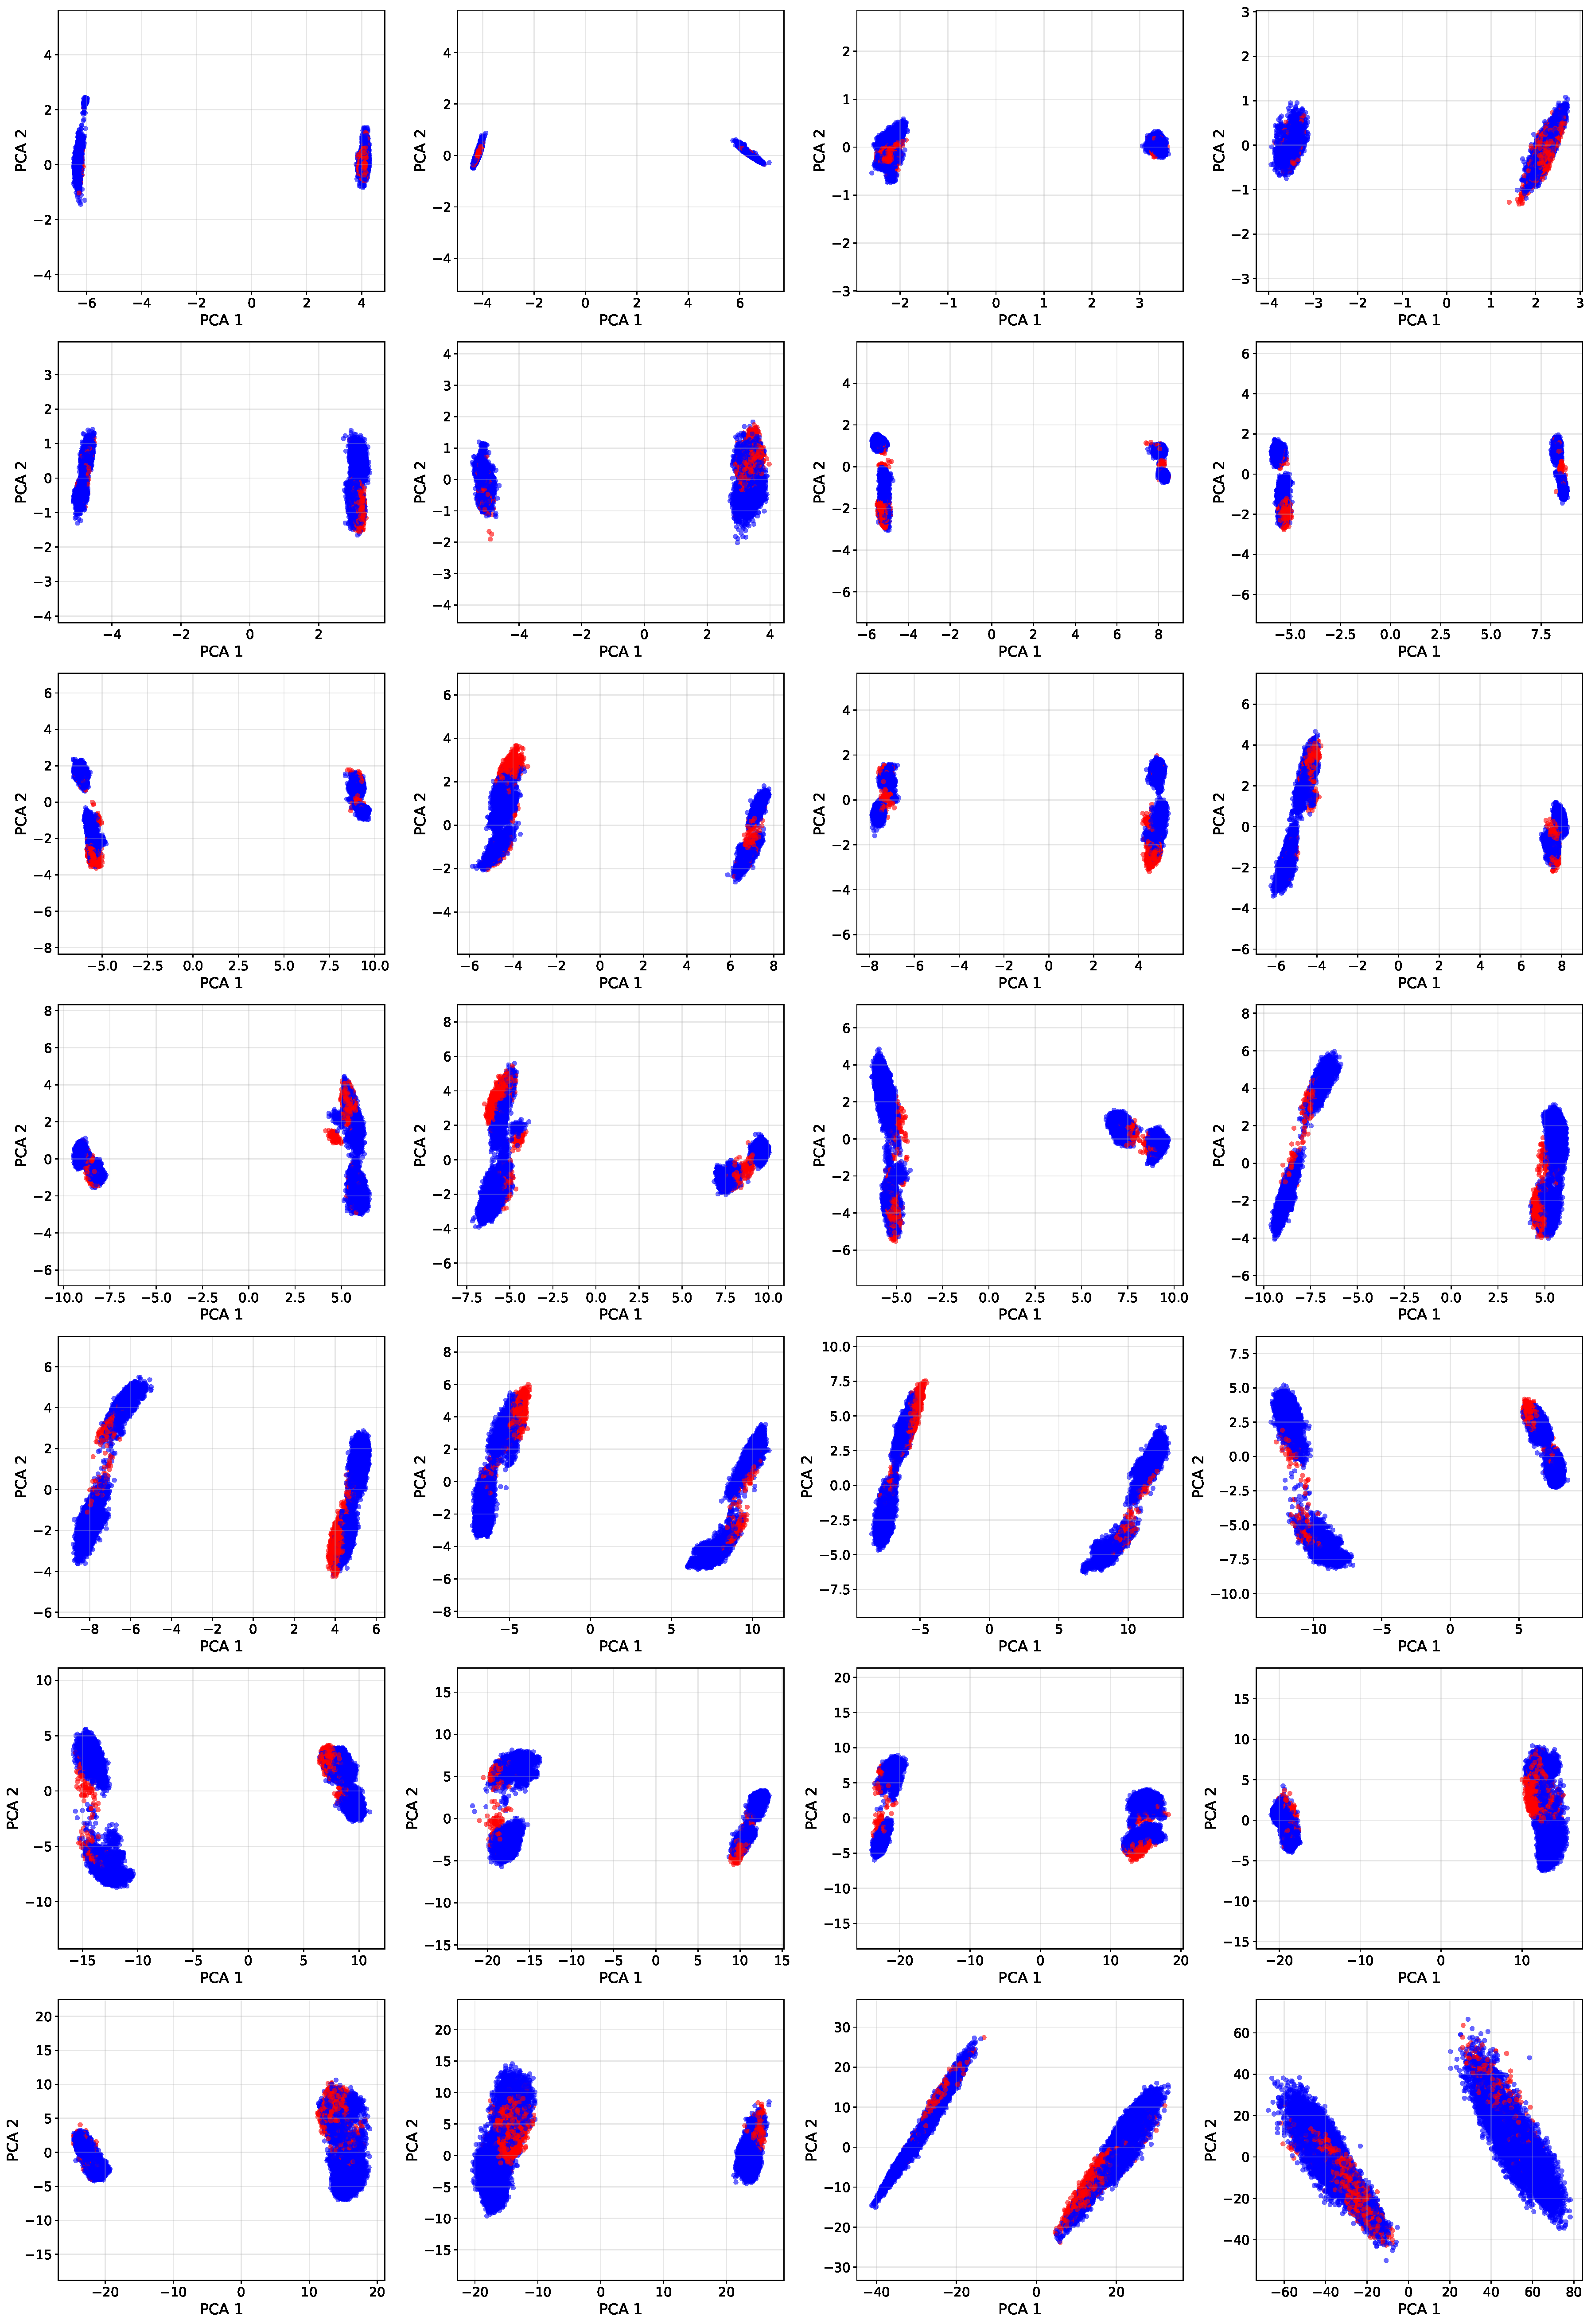
\includegraphics[width=\textwidth, height=1\textheight, keepaspectratio]{images/PCA_Plots/Qwen2.5-7B_belief_bank_facts_mlp_activations_PCA_CLEAN.pdf}
    \caption{PCA delle attivazioni MLP del layer di Qwen2.5-7B per Belief Bank Facts}

    \label{fig:qwen-pca-mlp-facts-full}
\end{figure}


\begin{figure}[H]
    \centering
    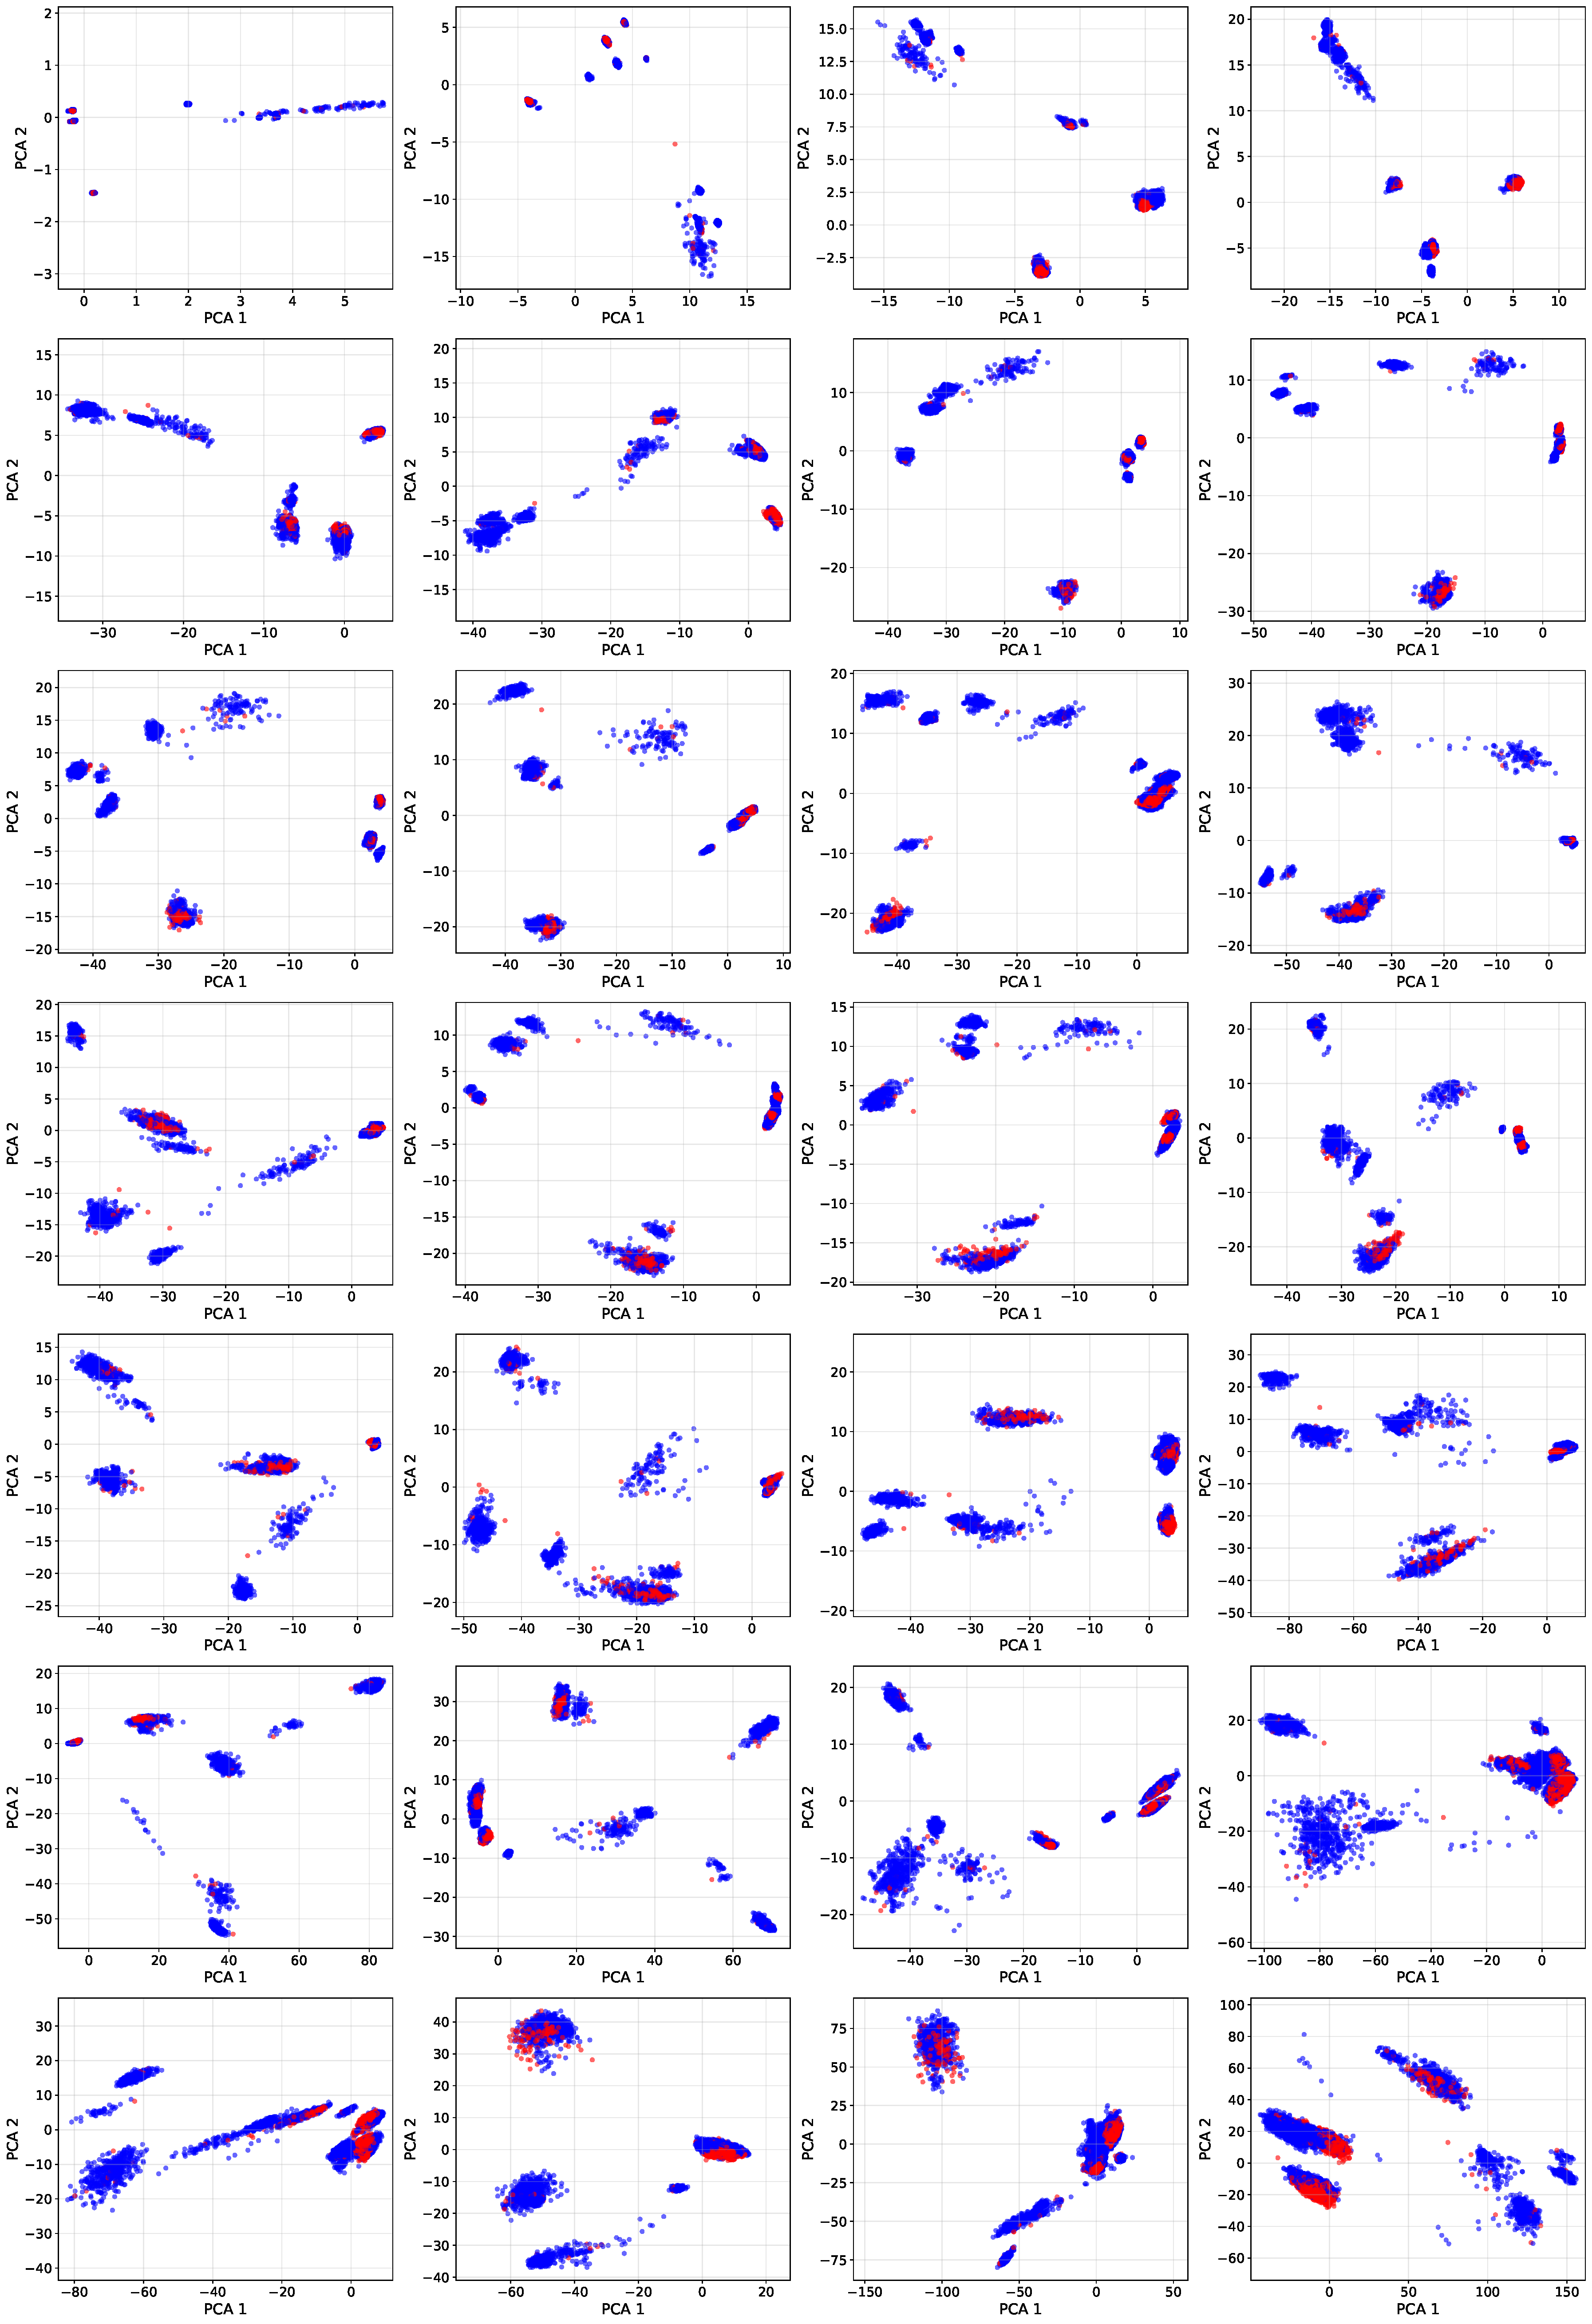
\includegraphics[width=\textwidth, height=1\textheight, keepaspectratio]{images/PCA_Plots/Falcon3-7B-Base_belief_bank_facts_attn_activations_PCA_CLEAN.pdf}
    \caption{PCA delle attivazioni Attention del layer di Falcon3-7B-Base per Belief Bank Facts}

    \label{fig:falcon-pca-attn-facts-full}
\end{figure}

\begin{figure}[H]
    \centering
    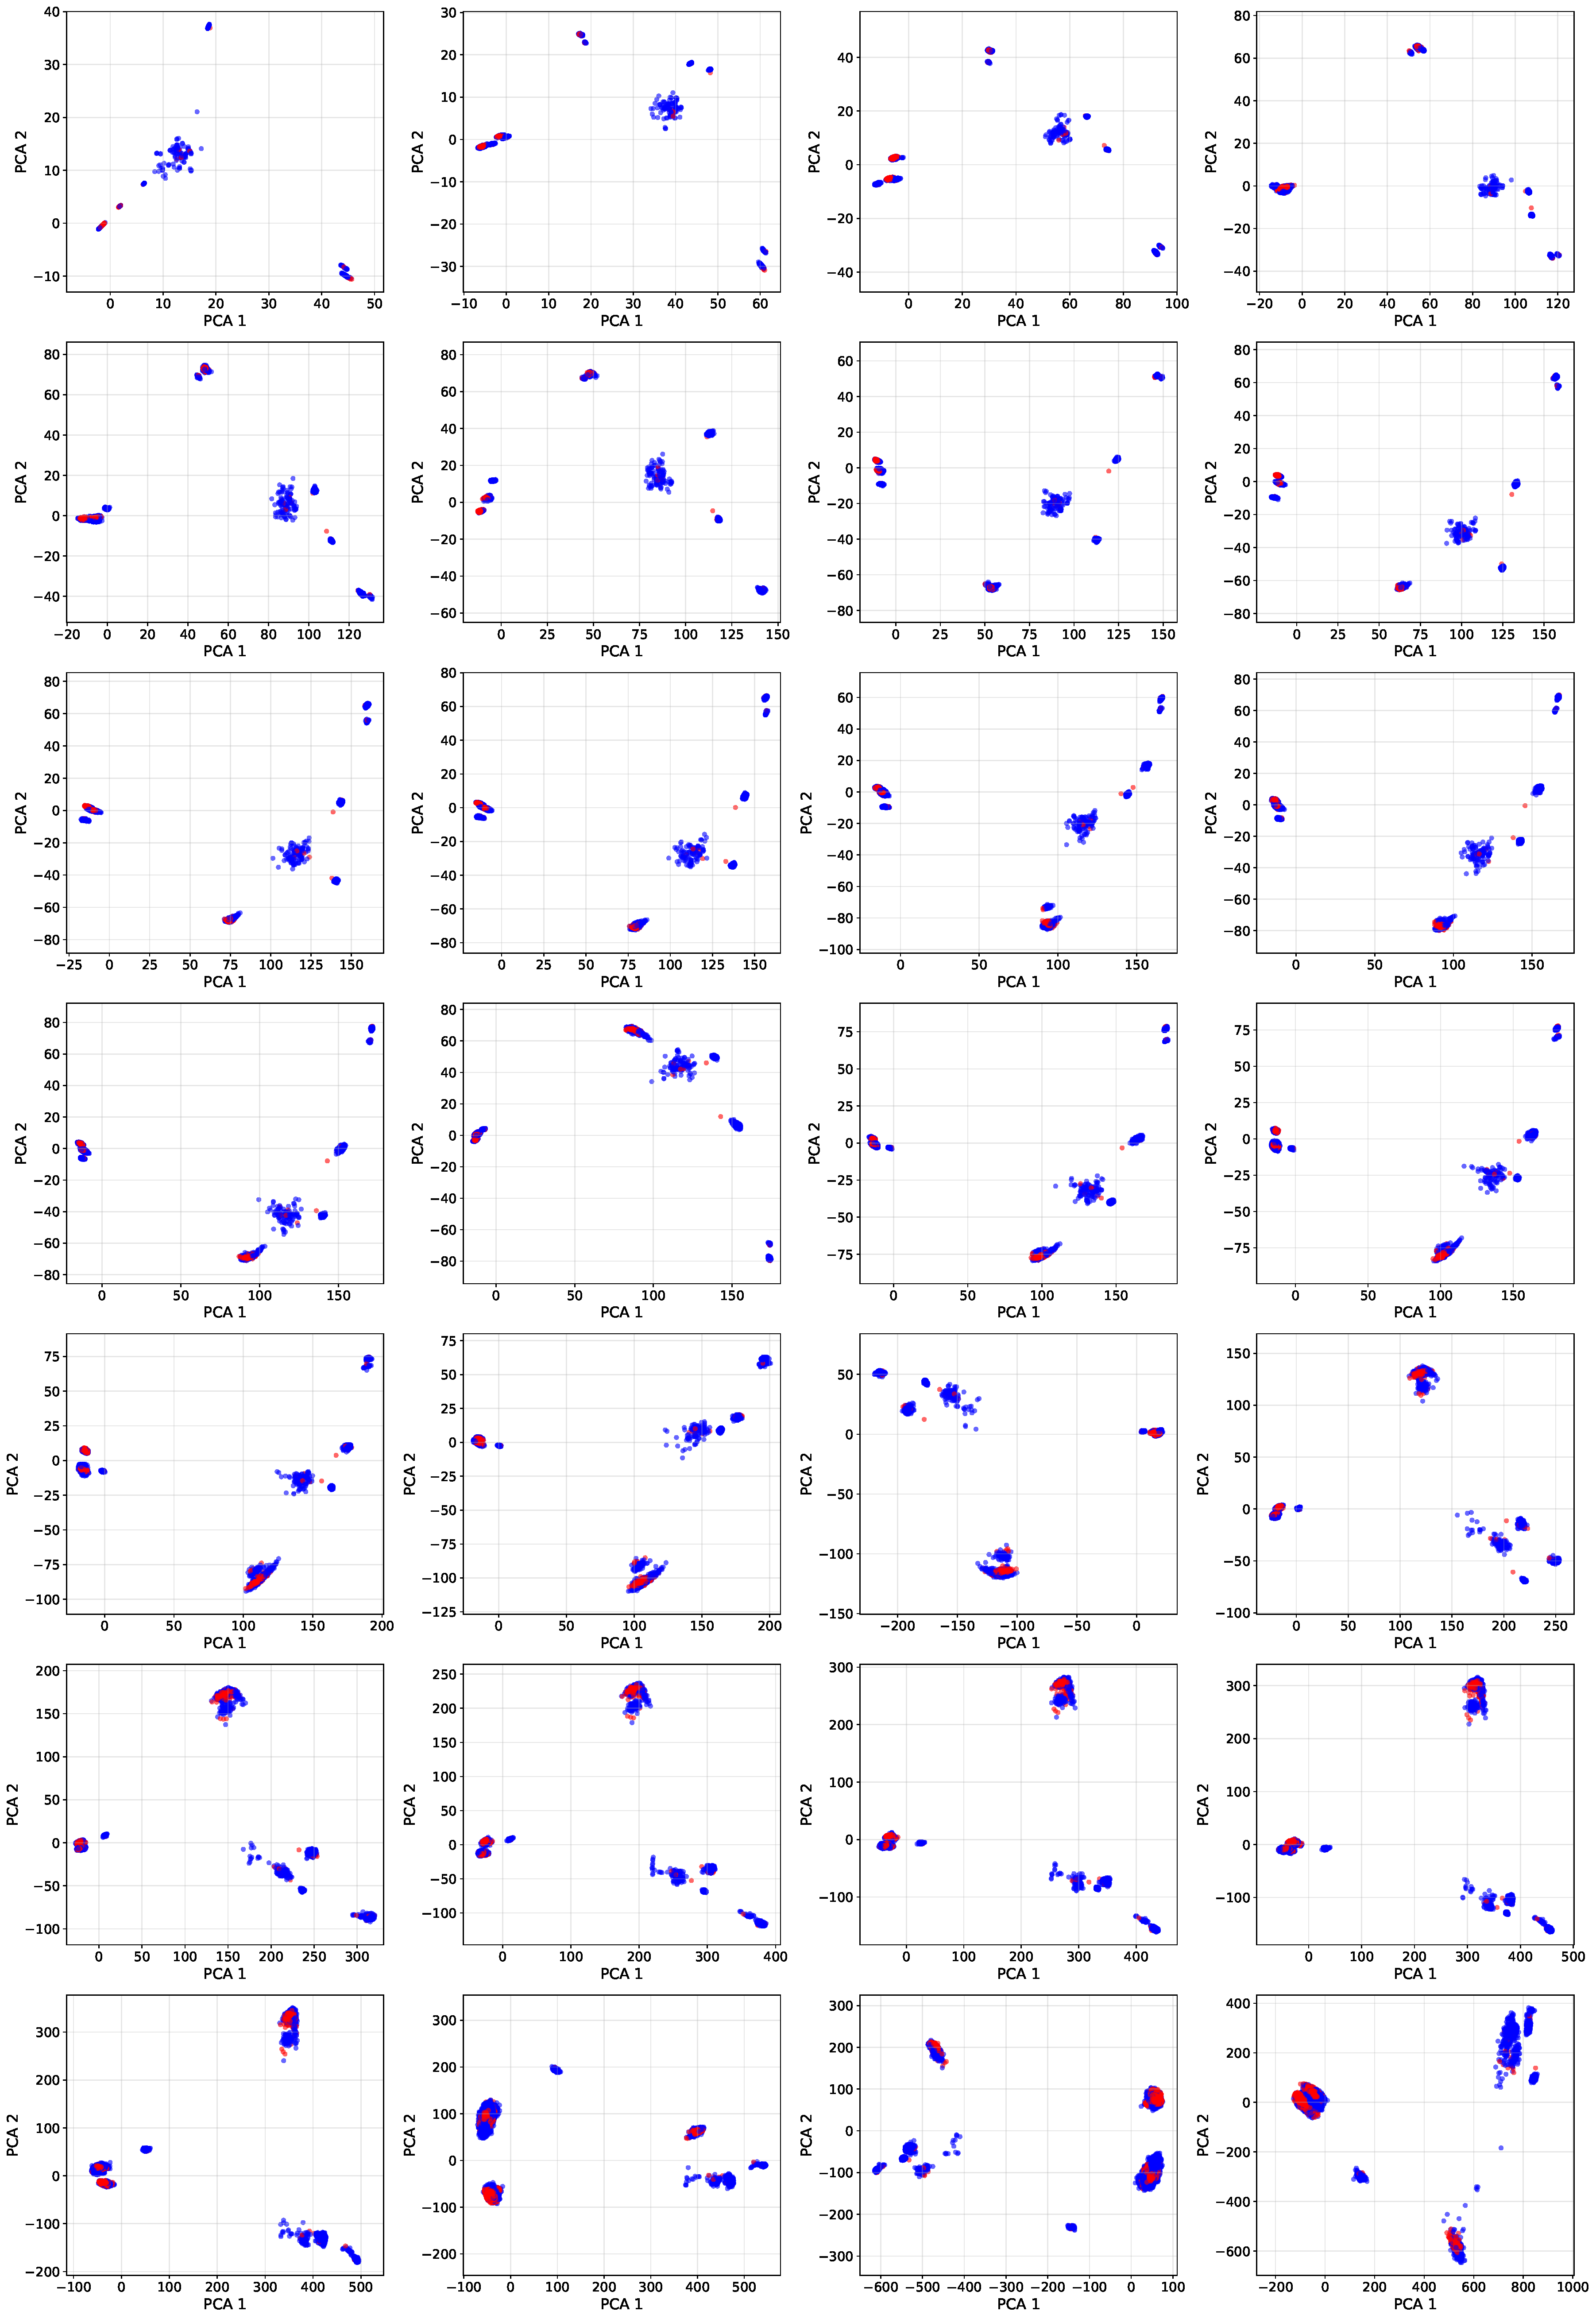
\includegraphics[width=\textwidth, height=1\textheight, keepaspectratio]{images/PCA_Plots/Falcon3-7B-Base_belief_bank_facts_hidden_activations_PCA_CLEAN.pdf}
    \caption{PCA delle attivazioni Hidden del layer di Falcon3-7B-Base per Belief Bank Facts}

    \label{fig:falcon-pca-hidden-facts-full}
\end{figure}

\begin{figure}[H]
    \centering
    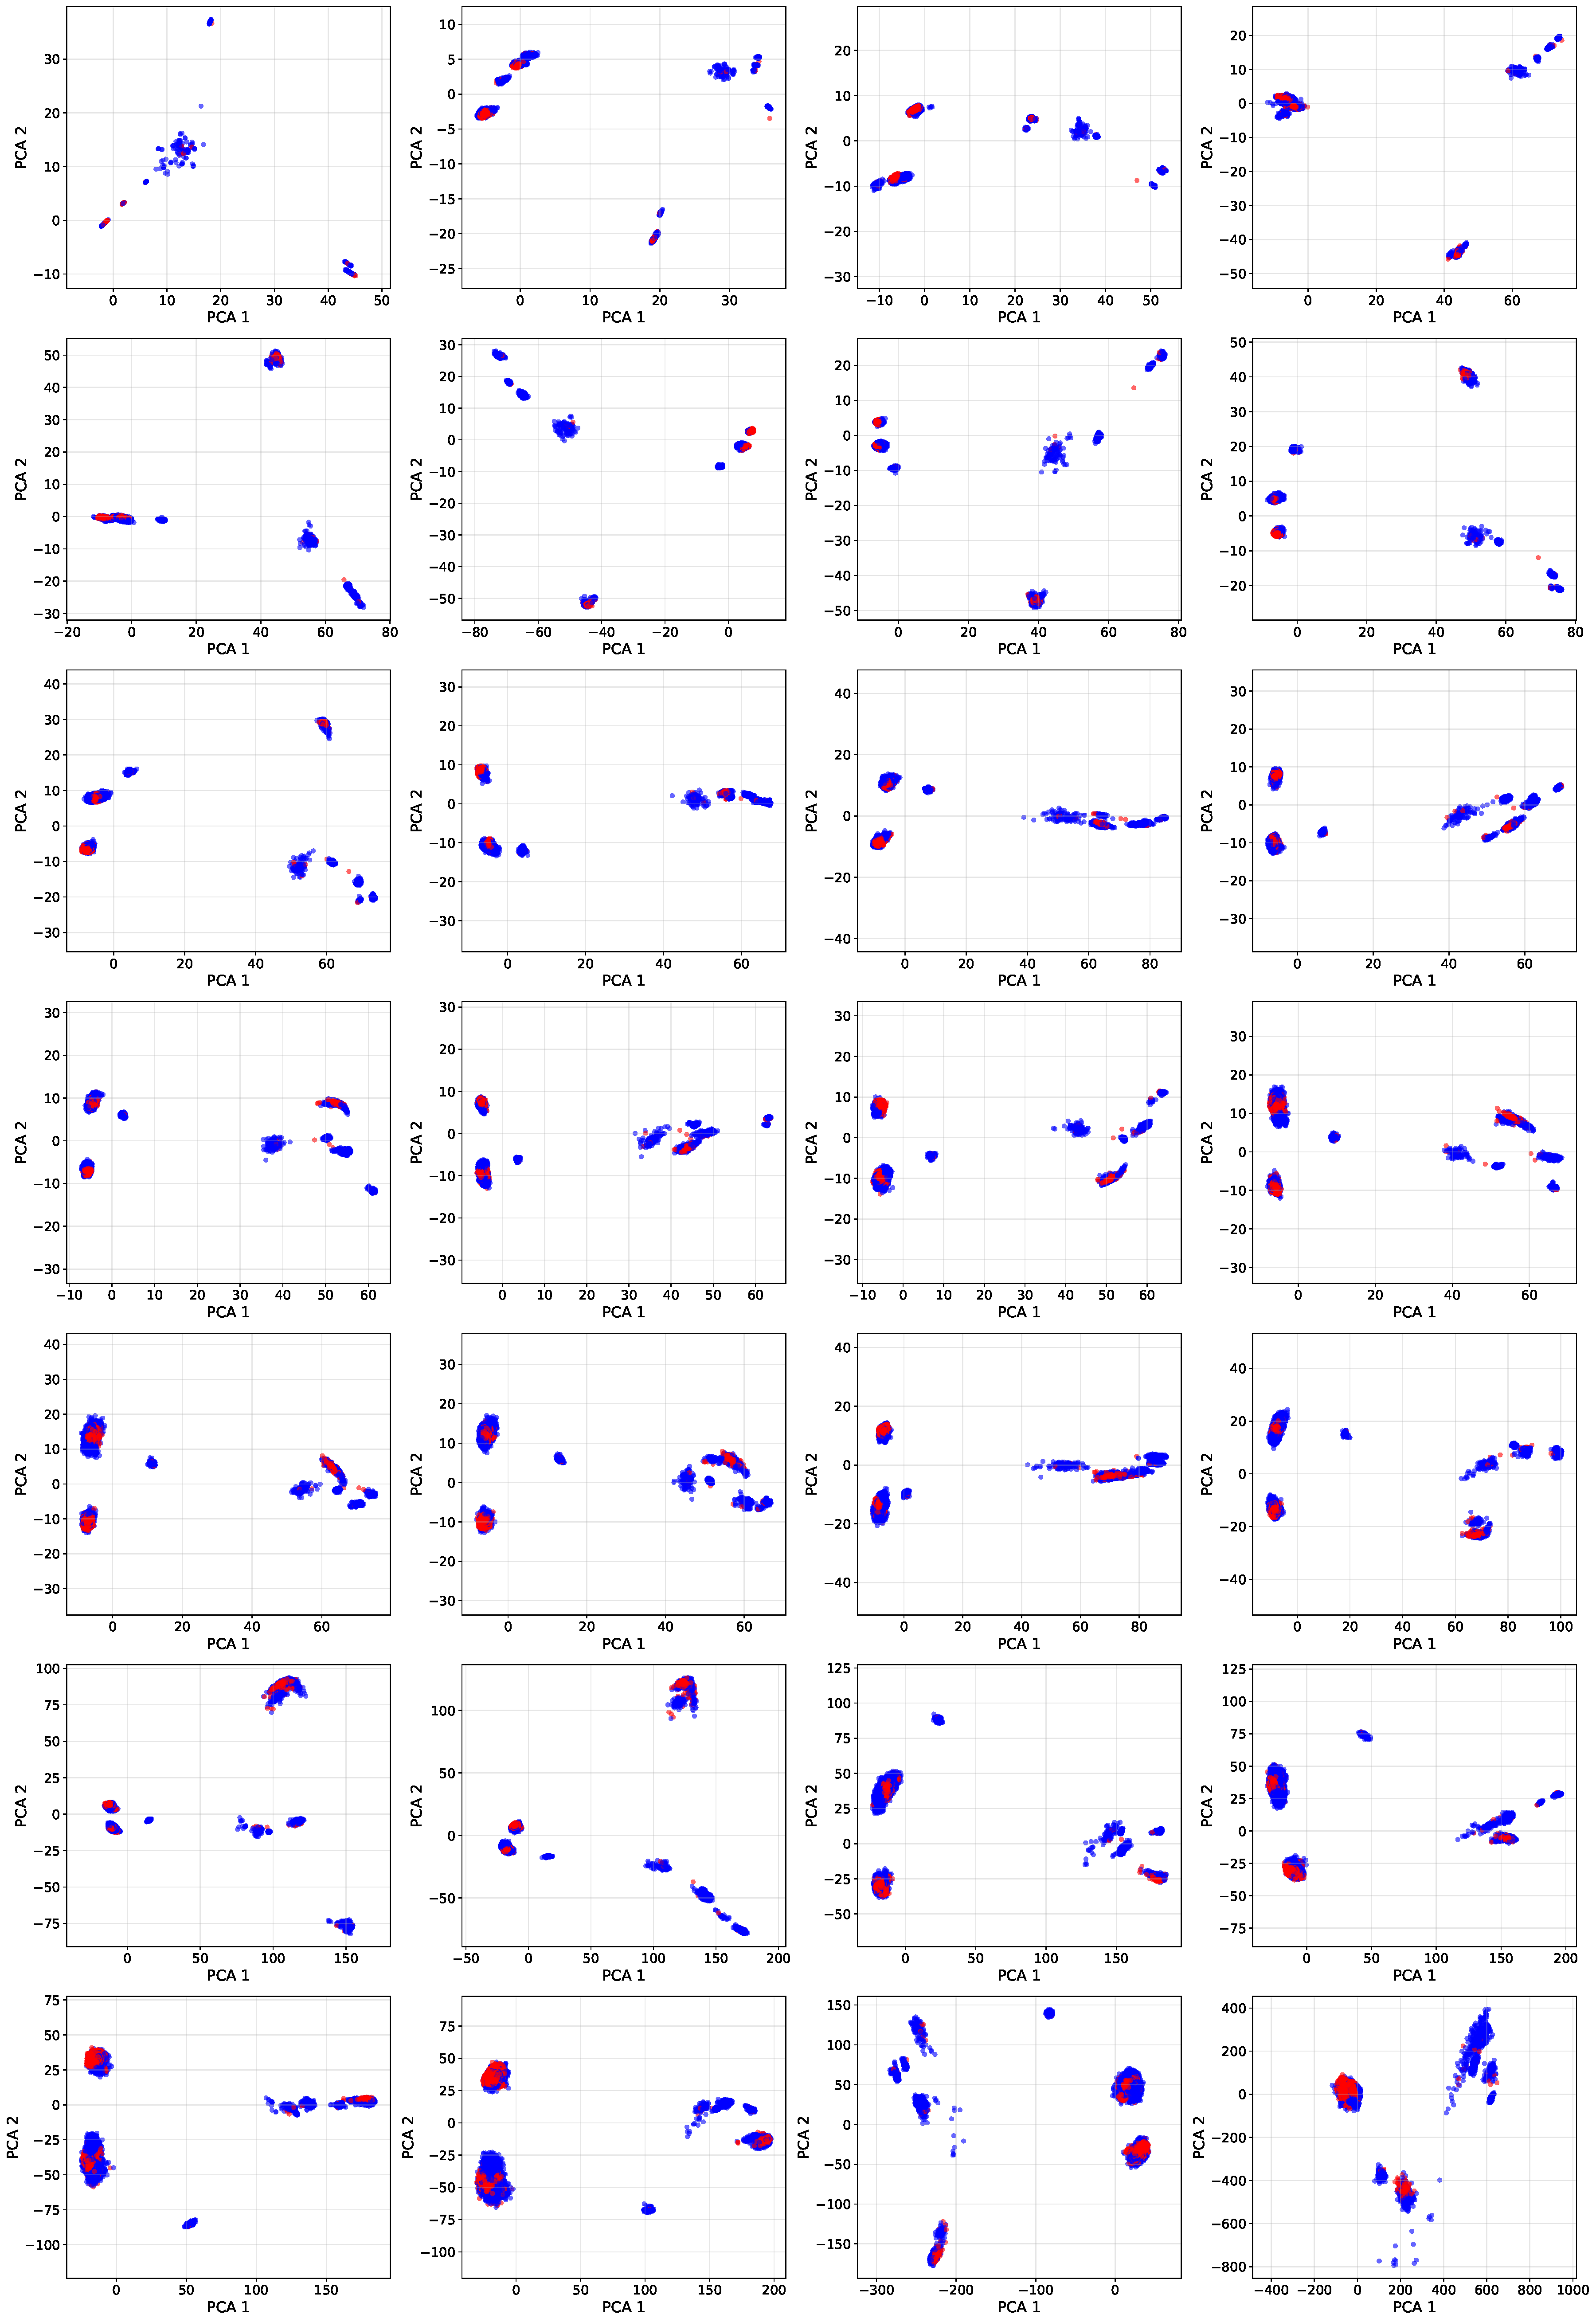
\includegraphics[width=\textwidth, height=1\textheight, keepaspectratio]{images/PCA_Plots/Falcon3-7B-Base_belief_bank_facts_mlp_activations_PCA_CLEAN.pdf}
    \caption{PCA delle attivazioni MLP del layer di Falcon3-7B-Base per Belief Bank Facts}

    \label{fig:falcon-pca-mlp-facts-full}
\end{figure}


\begin{figure}[H]
    \centering
    \includegraphics[width=\textwidth, height=1\textheight, keepaspectratio]{images/PCA_Plots/gemma-2-9b-it_belief_bank_facts_attn_activations_PCA_CLEAN.pdf}
    \label{fig:gemma-pca-attn-facts-full}
    \caption{PCA delle attivazioni Attention del layer di Gemma-2-9B-IT per Belief Bank Facts}
\end{figure}

\begin{figure}[H]
    \centering
    \includegraphics[width=\textwidth, height=1\textheight, keepaspectratio]{images/PCA_Plots/gemma-2-9b-it_belief_bank_facts_hidden_activations_PCA_CLEAN.pdf}
    \label{fig:gemma-pca-hidden-facts-full}
    \caption{PCA delle attivazioni Hidden del layer di Gemma-2-9B-IT per Belief Bank Facts}
\end{figure}

\begin{figure}[H]
    \centering
    \includegraphics[width=\textwidth, height=1\textheight, keepaspectratio]{images/PCA_Plots/gemma-2-9b-it_belief_bank_facts_mlp_activations_PCA_CLEAN.pdf}
    \label{fig:gemma-pca-mlp-facts-full}
    \caption{PCA delle attivazioni MLP del layer di Gemma-2-9B-IT per Belief Bank Facts}
\end{figure}

\begin{figure}[H]
    \centering
    \includegraphics[width=\textwidth, height=1\textheight, keepaspectratio]{images/PCA_Plots/Llama-3.1-8B-Instruct_belief_bank_facts_attn_activations_PCA_CLEAN.pdf}
    \label{fig:llama-pca-attn-facts-full}
    \caption{PCA delle attivazioni Attention del layer di Llama-3.1-8B-Instruct per Belief Bank Facts}
\end{figure}

\begin{figure}[H]
    \centering
    \includegraphics[width=\textwidth, height=1\textheight, keepaspectratio]{images/PCA_Plots/Llama-3.1-8B-Instruct_belief_bank_facts_hidden_activations_PCA_CLEAN.pdf}
    \label{fig:llama-pca-hidden-facts-full}
    \caption{PCA delle attivazioni Hidden del layer di Llama-3.1-8B-Instruct per Belief Bank Facts}
\end{figure}

\begin{figure}[H]
    \centering
    \includegraphics[width=\textwidth, height=1\textheight, keepaspectratio]{images/PCA_Plots/Llama-3.1-8B-Instruct_belief_bank_facts_mlp_activations_PCA_CLEAN.pdf}
    \label{fig:llama-pca-mlp-facts-full}
    \caption{PCA delle attivazioni MLP del layer di Llama-3.1-8B-Instruct per Belief Bank Facts}
\end{figure}


\begin{figure}[H]
    \centering
    \includegraphics[width=\textwidth, height=1\textheight, keepaspectratio]{images/PCA_Plots/gemma-2-9b-it_belief_bank_constraints_attn_activations_PCA_CLEAN.pdf}
    \label{fig:gemma-pca-attn-constraints-full}
    \caption{PCA delle attivazioni Attention del layer di Gemma-2-9B-IT per Belief Bank Constraints}
\end{figure}

\begin{figure}[H]
    \centering
    \includegraphics[width=\textwidth, height=1\textheight, keepaspectratio]{images/PCA_Plots/gemma-2-9b-it_belief_bank_constraints_hidden_activations_PCA_CLEAN.pdf}
    \label{fig:gemma-pca-hidden-constraints-full}
    \caption{PCA delle attivazioni Hidden del layer di Gemma-2-9B-IT per Belief Bank Constraints}
\end{figure}

\begin{figure}[H]
    \centering
    \includegraphics[width=\textwidth, height=1\textheight, keepaspectratio]{images/PCA_Plots/gemma-2-9b-it_belief_bank_constraints_mlp_activations_PCA_CLEAN.pdf}
    \label{fig:gemma-pca-mlp-constraints-full}
    \caption{PCA delle attivazioni MLP del layer di Gemma-2-9B-IT per Belief Bank Constraints}
\end{figure}


\begin{figure}[H]
    \centering
    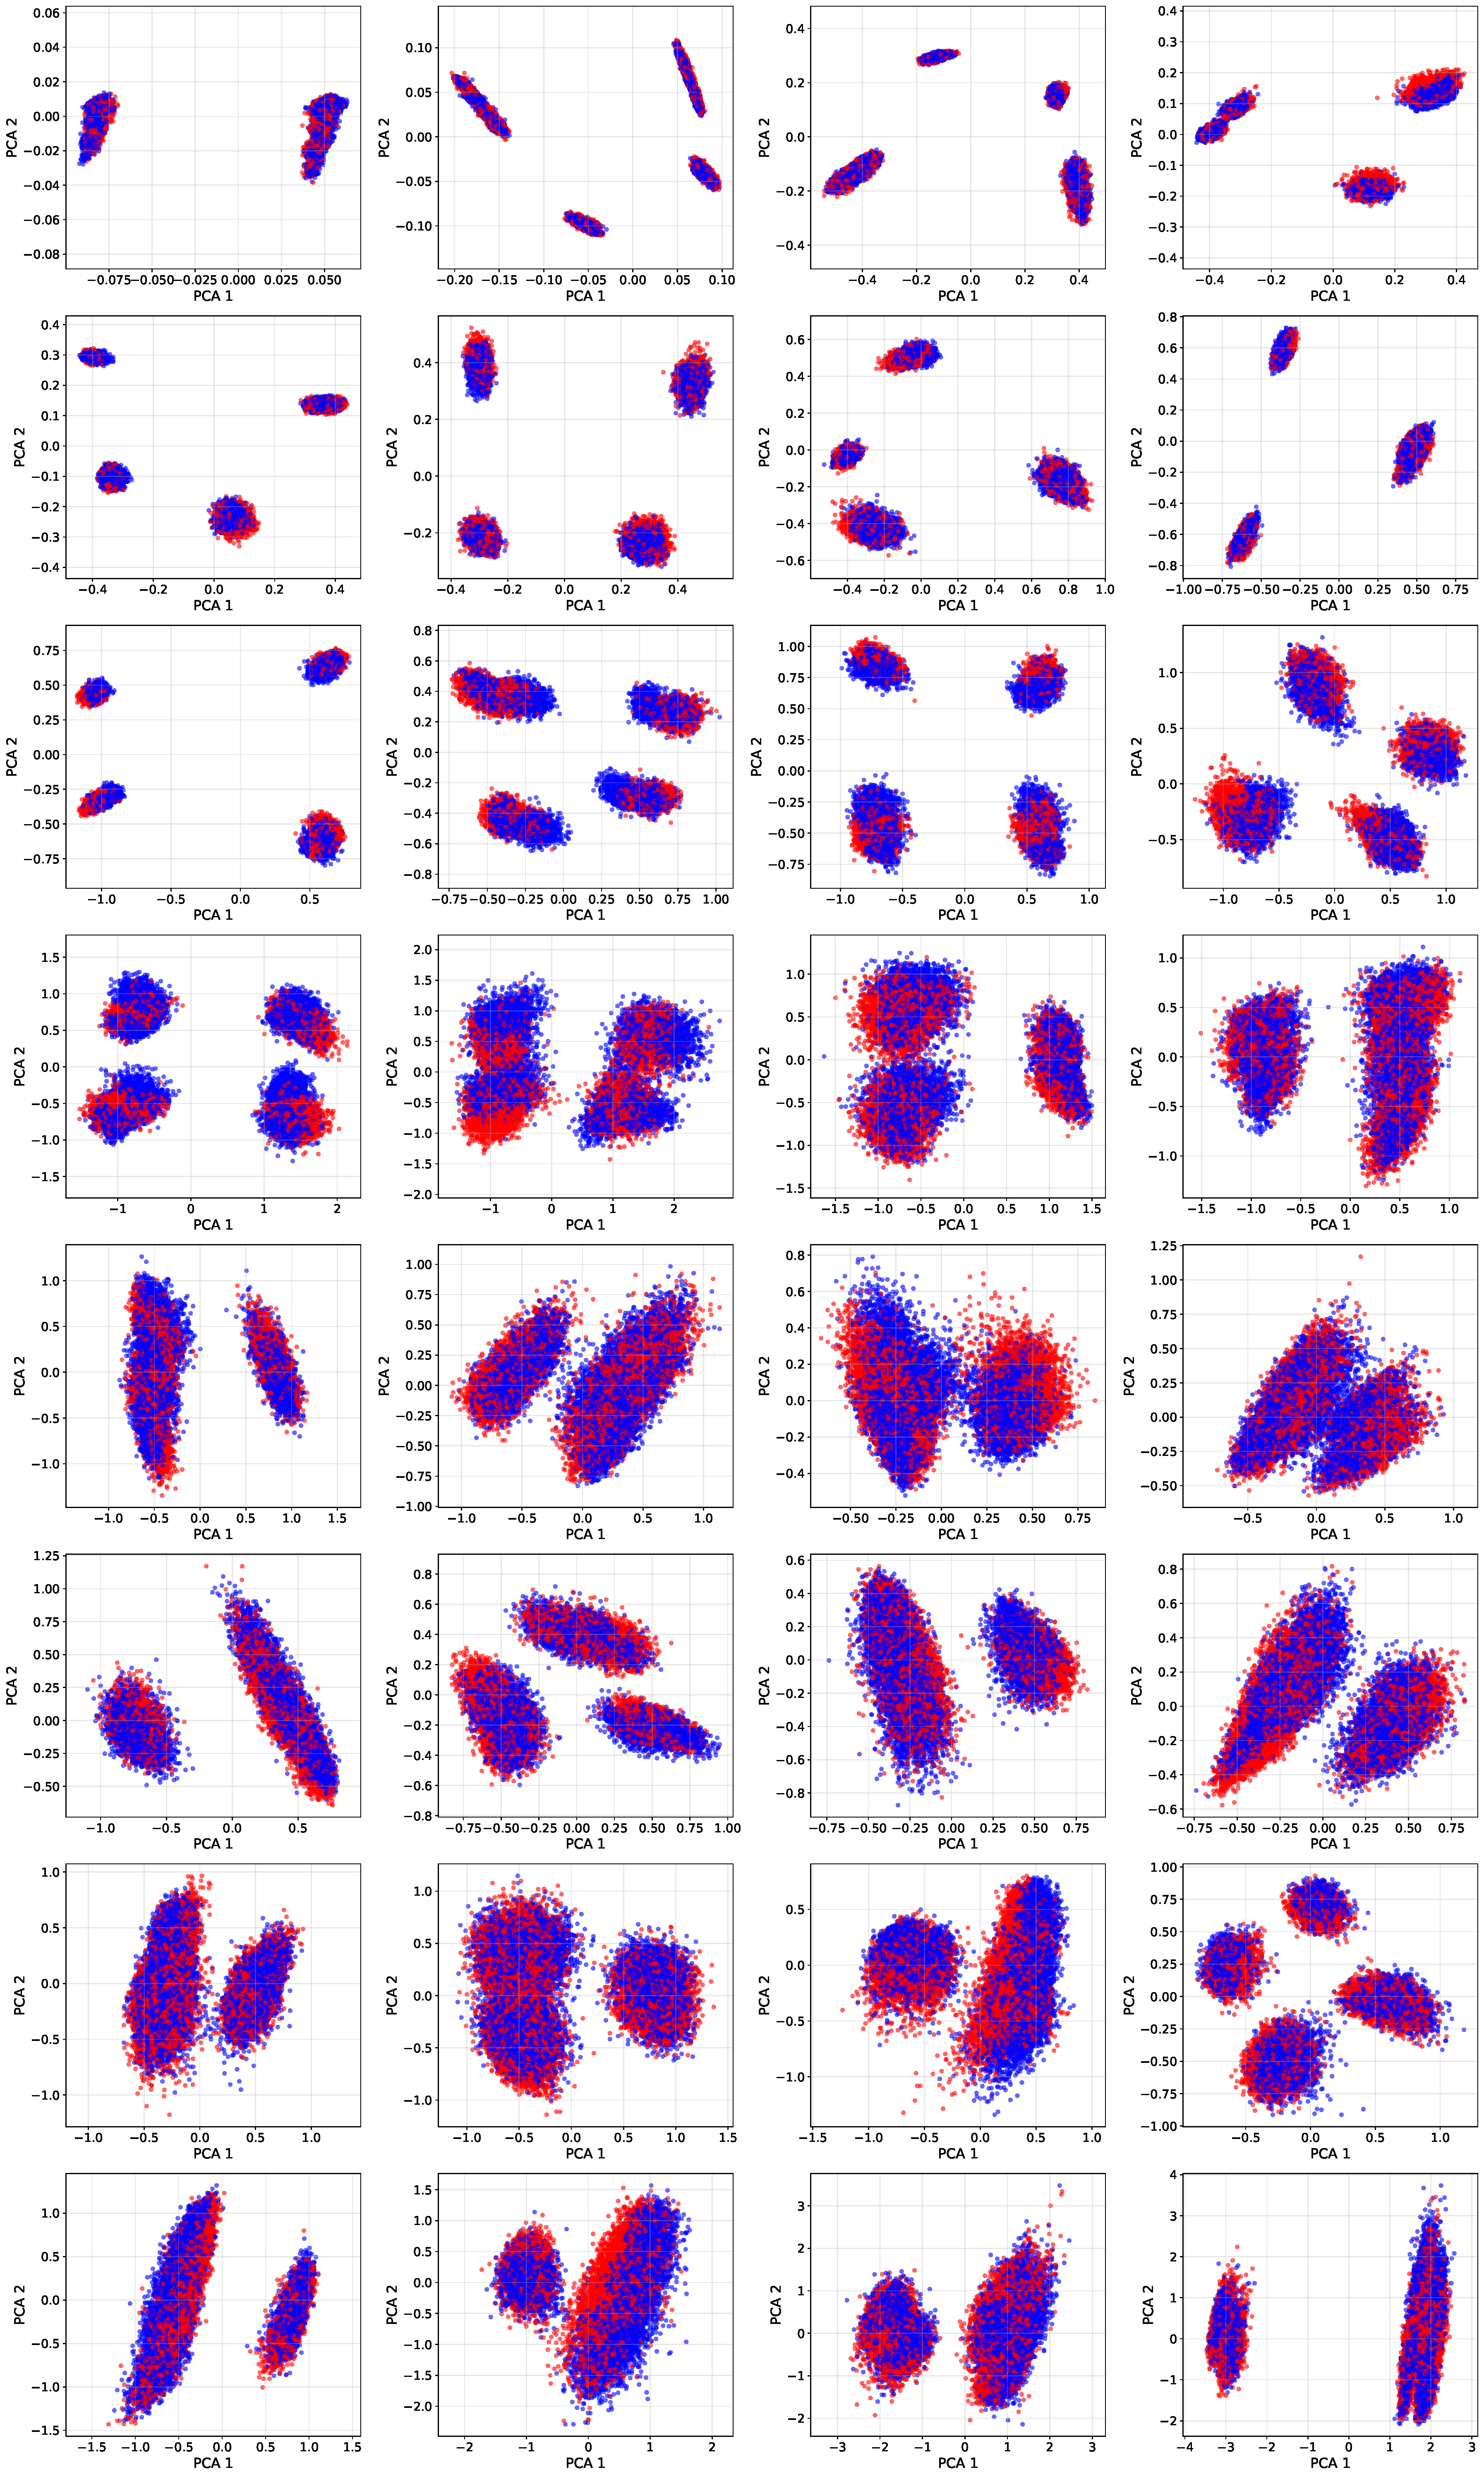
\includegraphics[width=\textwidth, height=1\textheight, keepaspectratio]{images/PCA_Plots/Llama-3.1-8B-Instruct_belief_bank_constraints_attn_activations_PCA_CLEAN.pdf}
    \label{fig:llama-pca-attn-constraints-full}
    \caption{PCA delle attivazioni Attention del layer di Llama-3.1-8B-Instruct per Belief Bank Constraints}
\end{figure}

\begin{figure}[H]
    \centering
    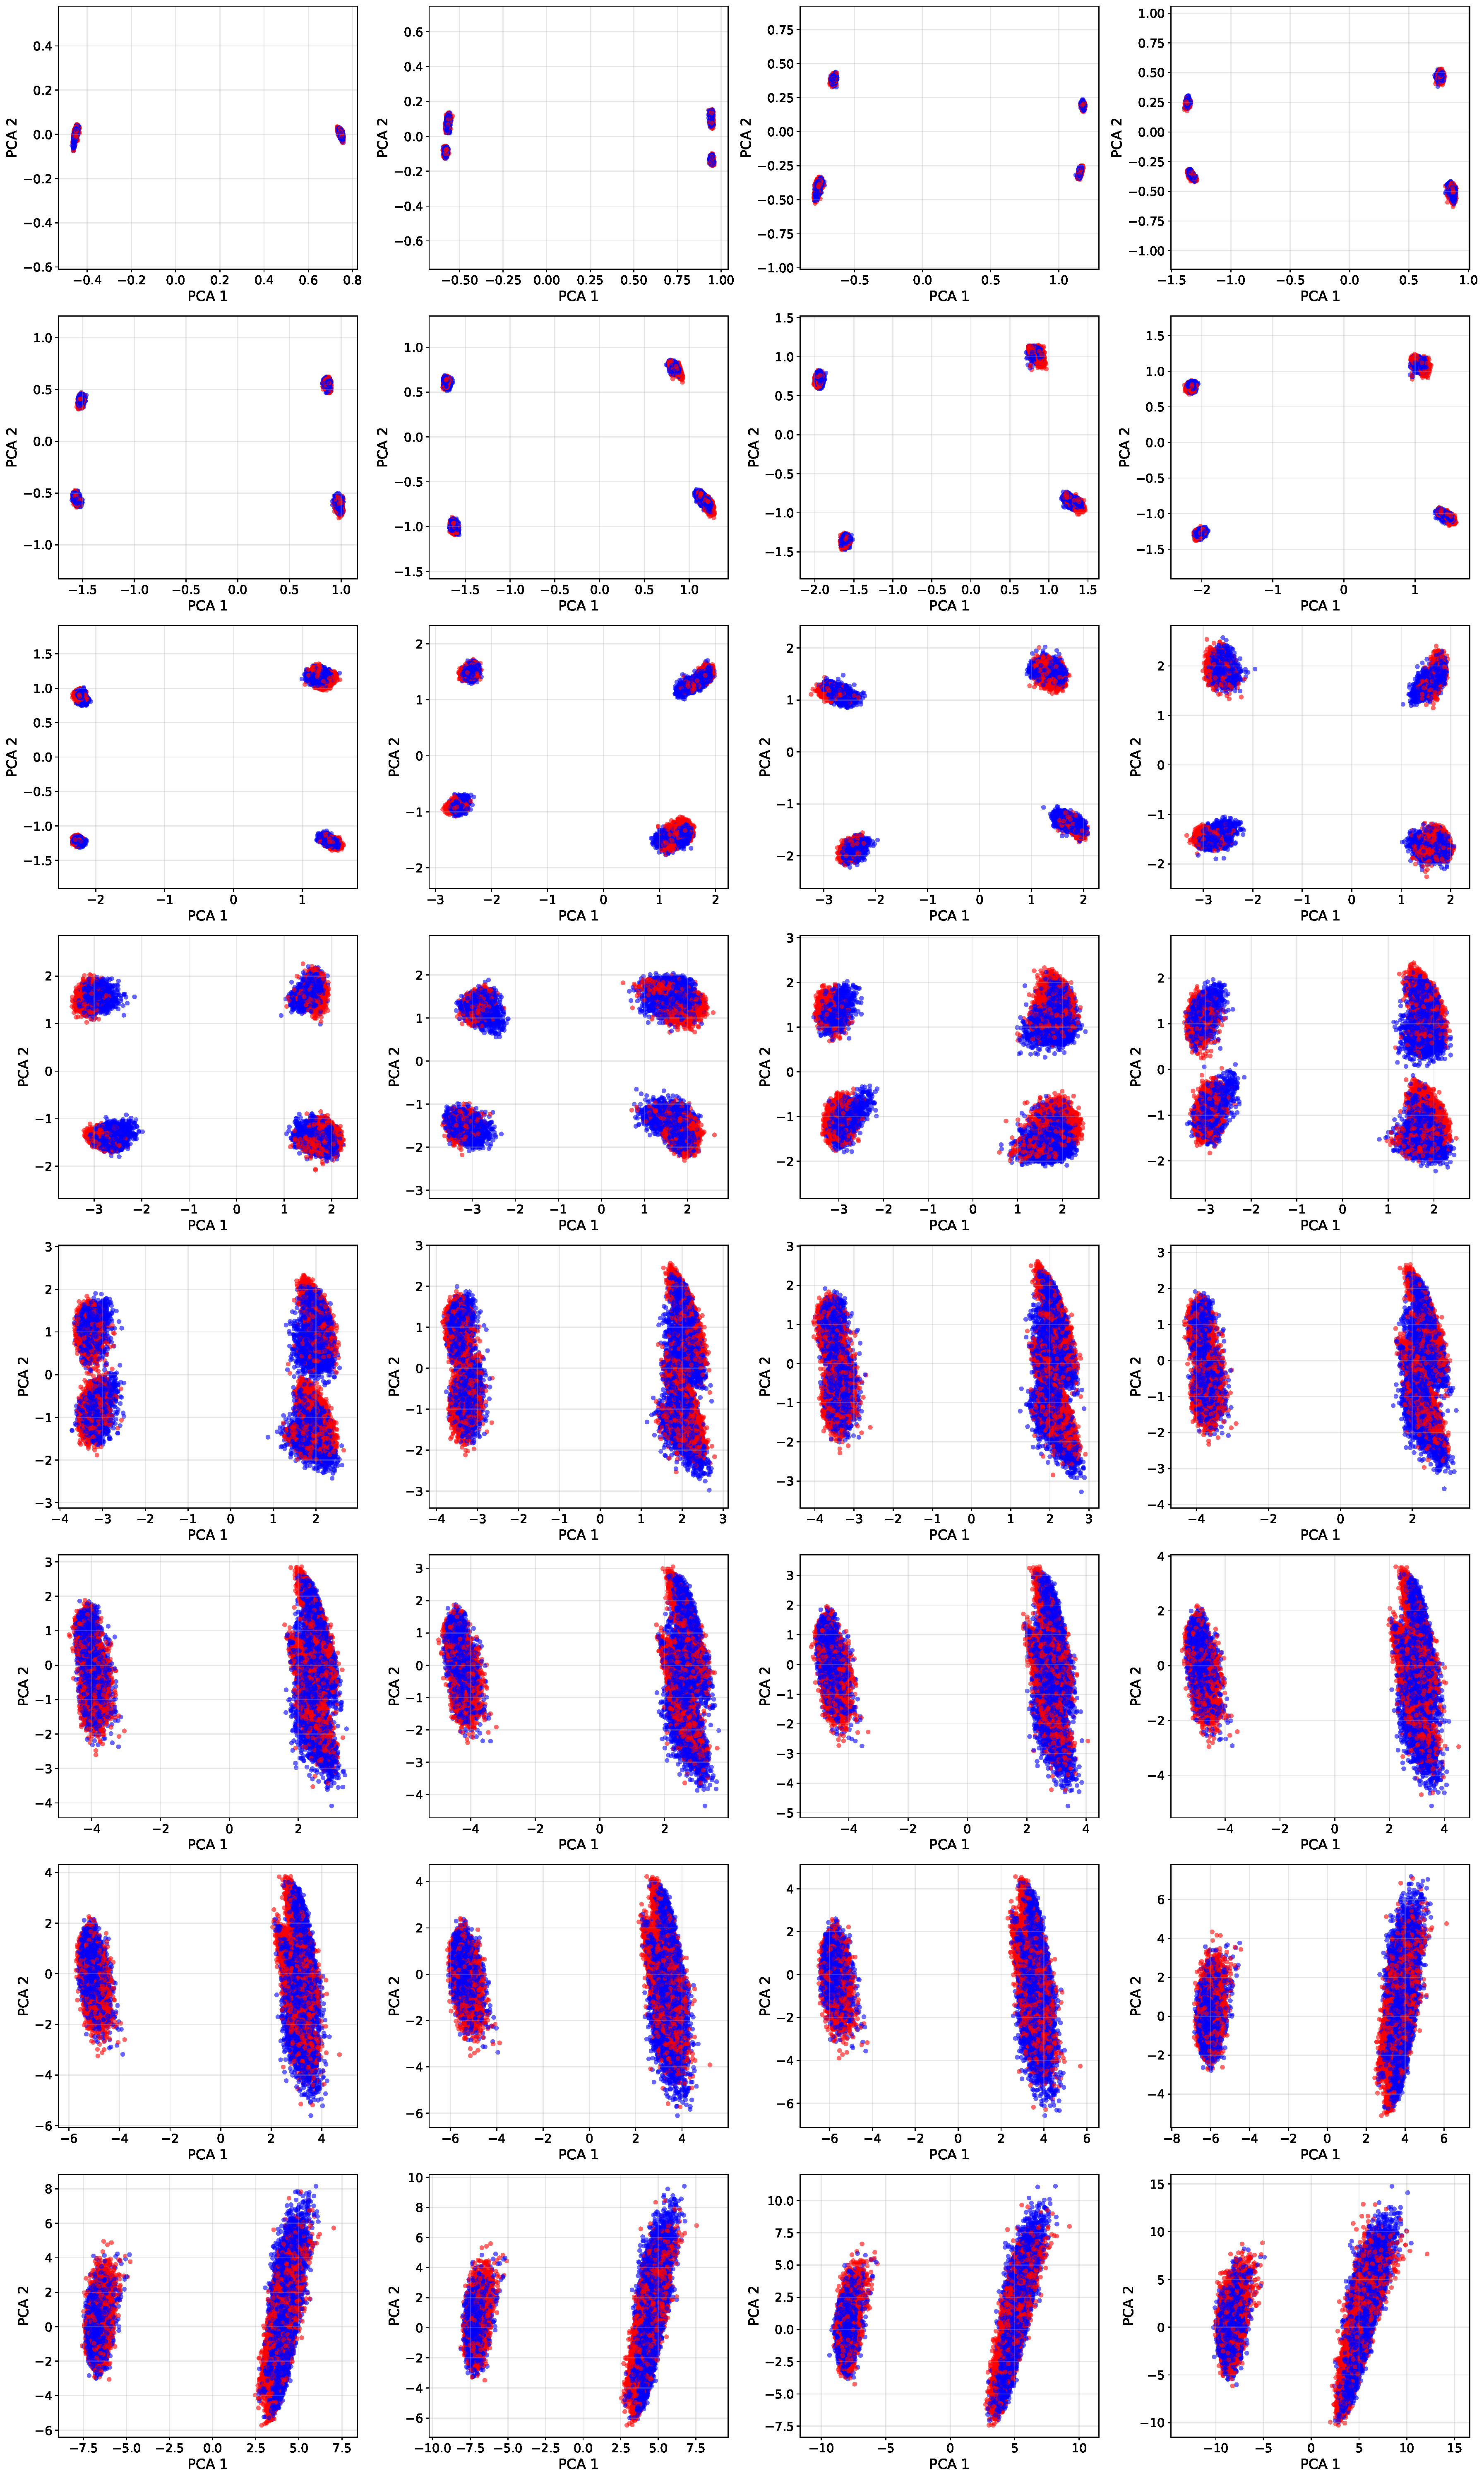
\includegraphics[width=\textwidth, height=1\textheight, keepaspectratio]{images/PCA_Plots/Llama-3.1-8B-Instruct_belief_bank_constraints_hidden_activations_PCA_CLEAN.pdf}
    \label{fig:llama-pca-hidden-constraints-full}
    \caption{PCA delle attivazioni Hidden del layer di Llama-3.1-8B-Instruct per Belief Bank Constraints}
\end{figure}


\begin{figure}[H]
    \centering
    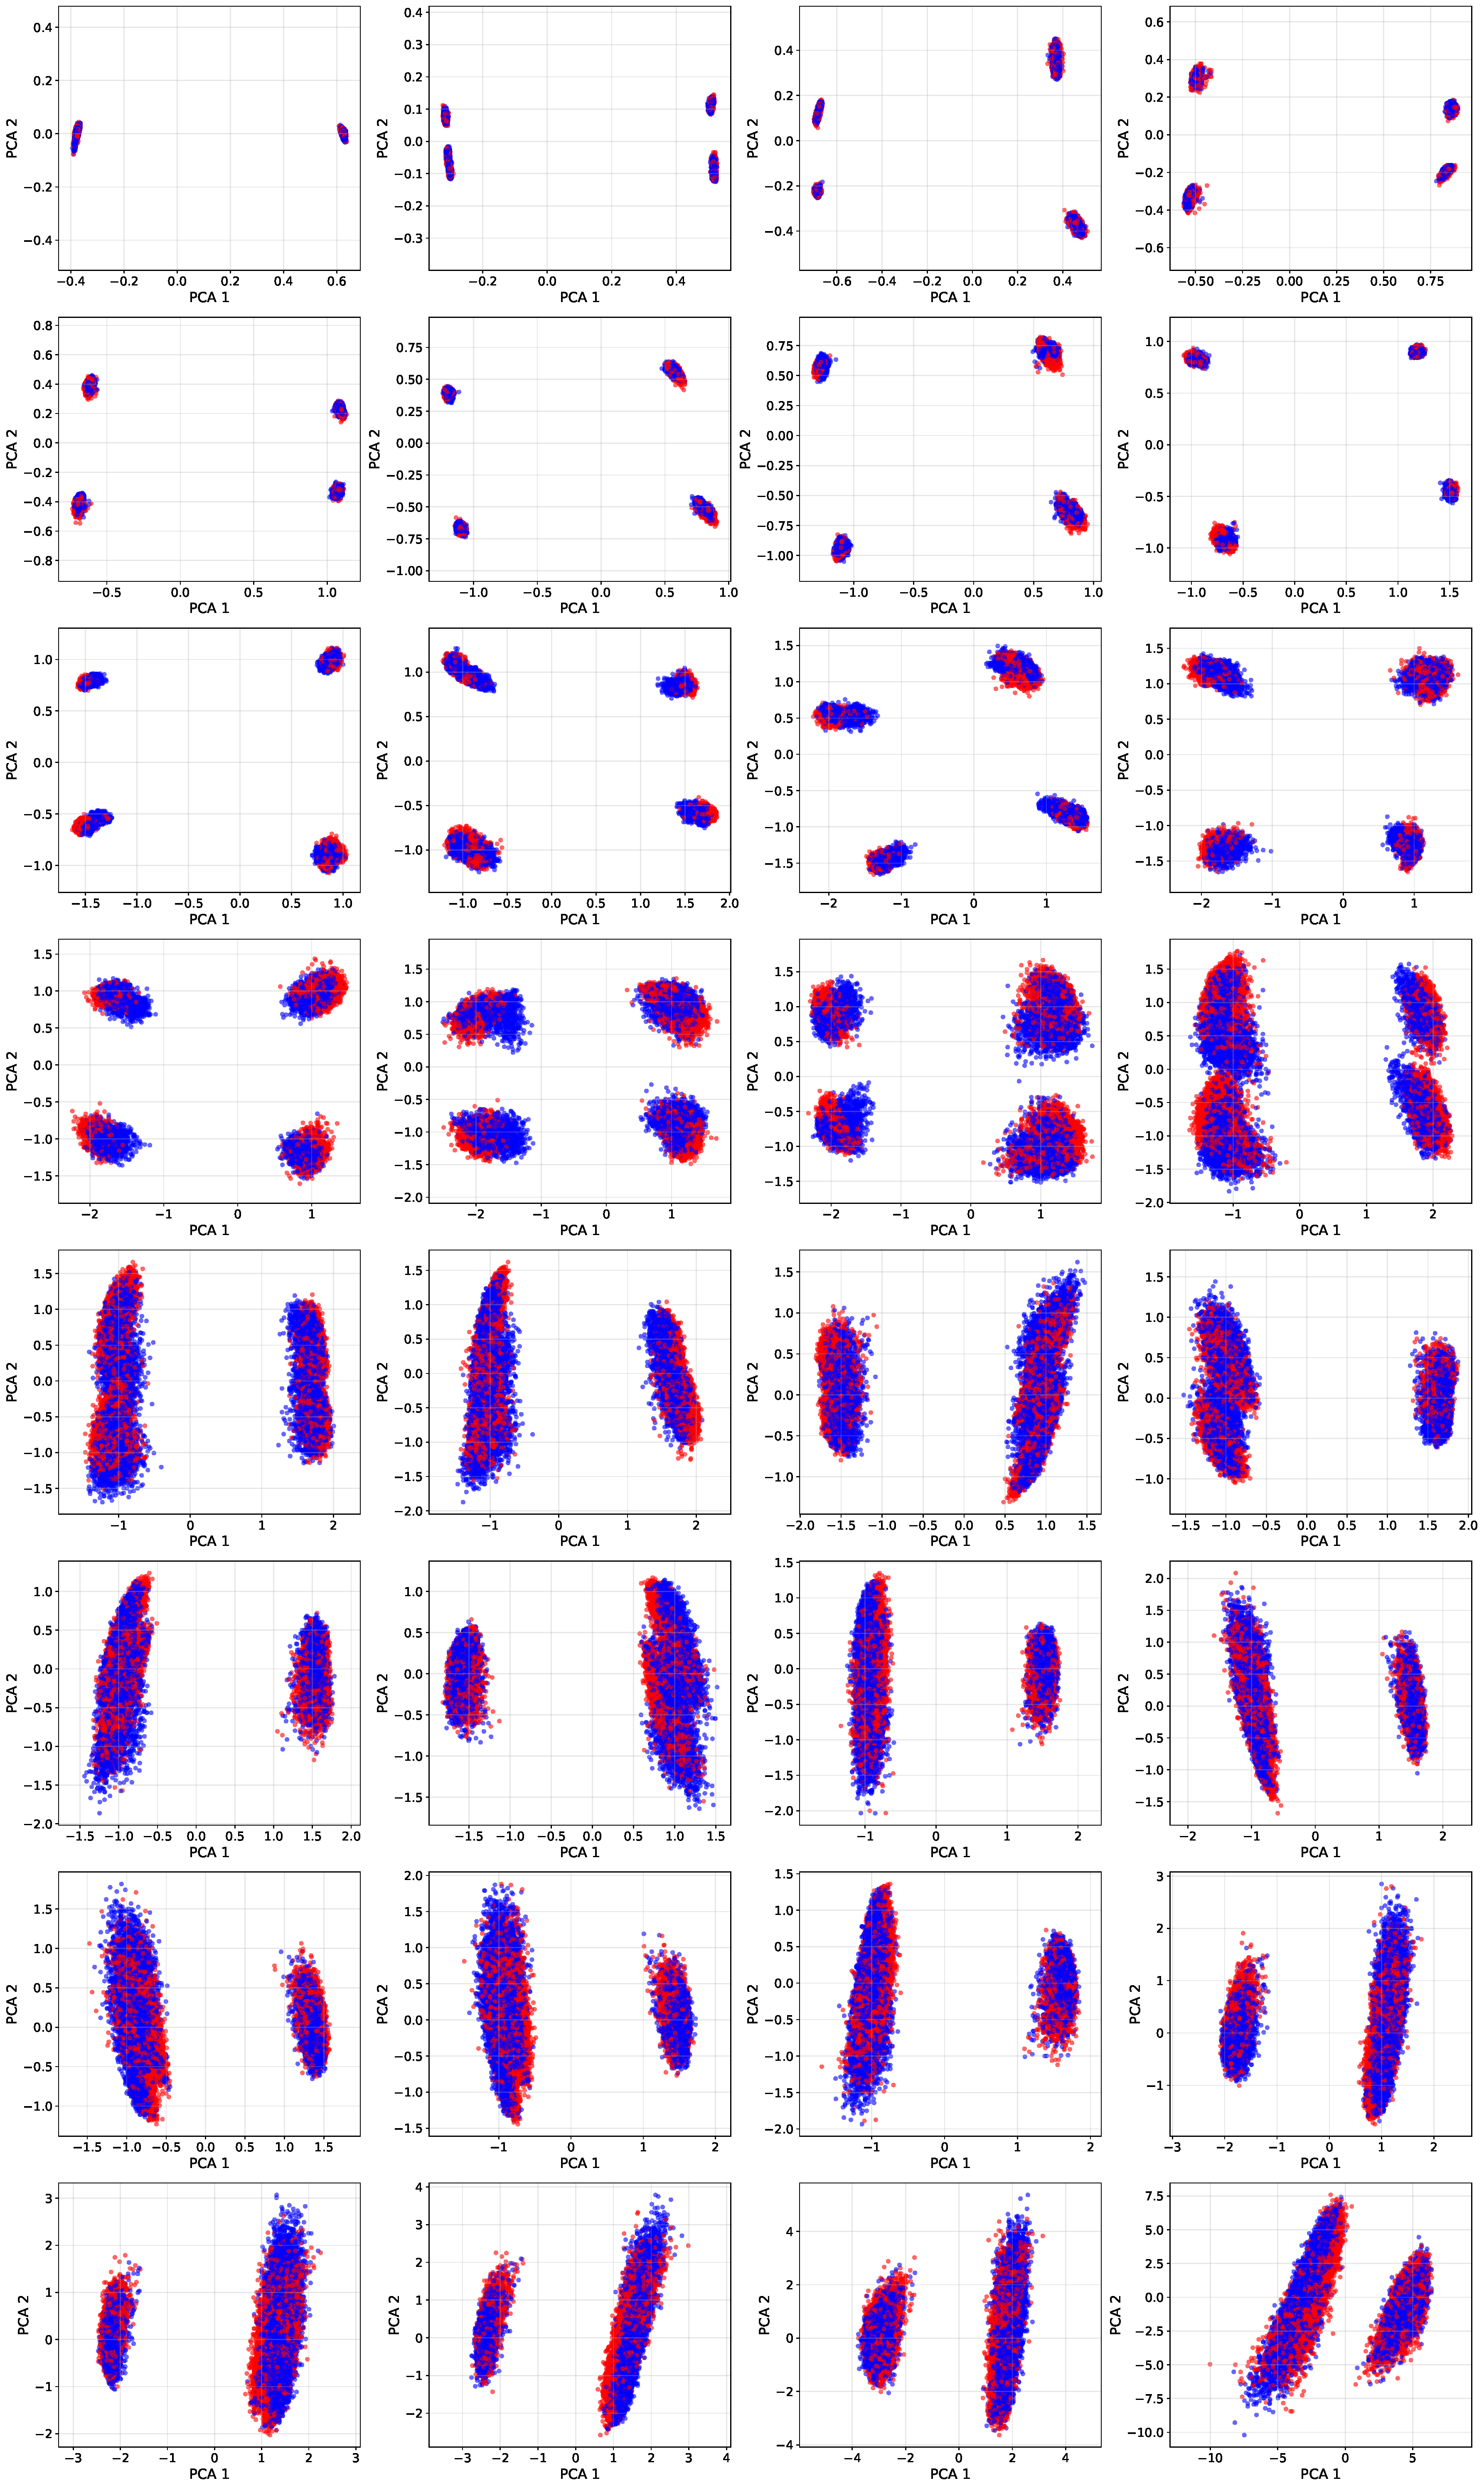
\includegraphics[width=\textwidth, height=1\textheight, keepaspectratio]{images/PCA_Plots/Llama-3.1-8B-Instruct_belief_bank_constraints_mlp_activations_PCA_CLEAN.pdf}
    \label{fig:llama-pca-mlp-constraints-full}
    \caption{PCA delle attivazioni MLP del layer di Llama-3.1-8B-Instruct per Belief Bank Constraints}
\end{figure}


\begin{figure}[H]
    \centering
    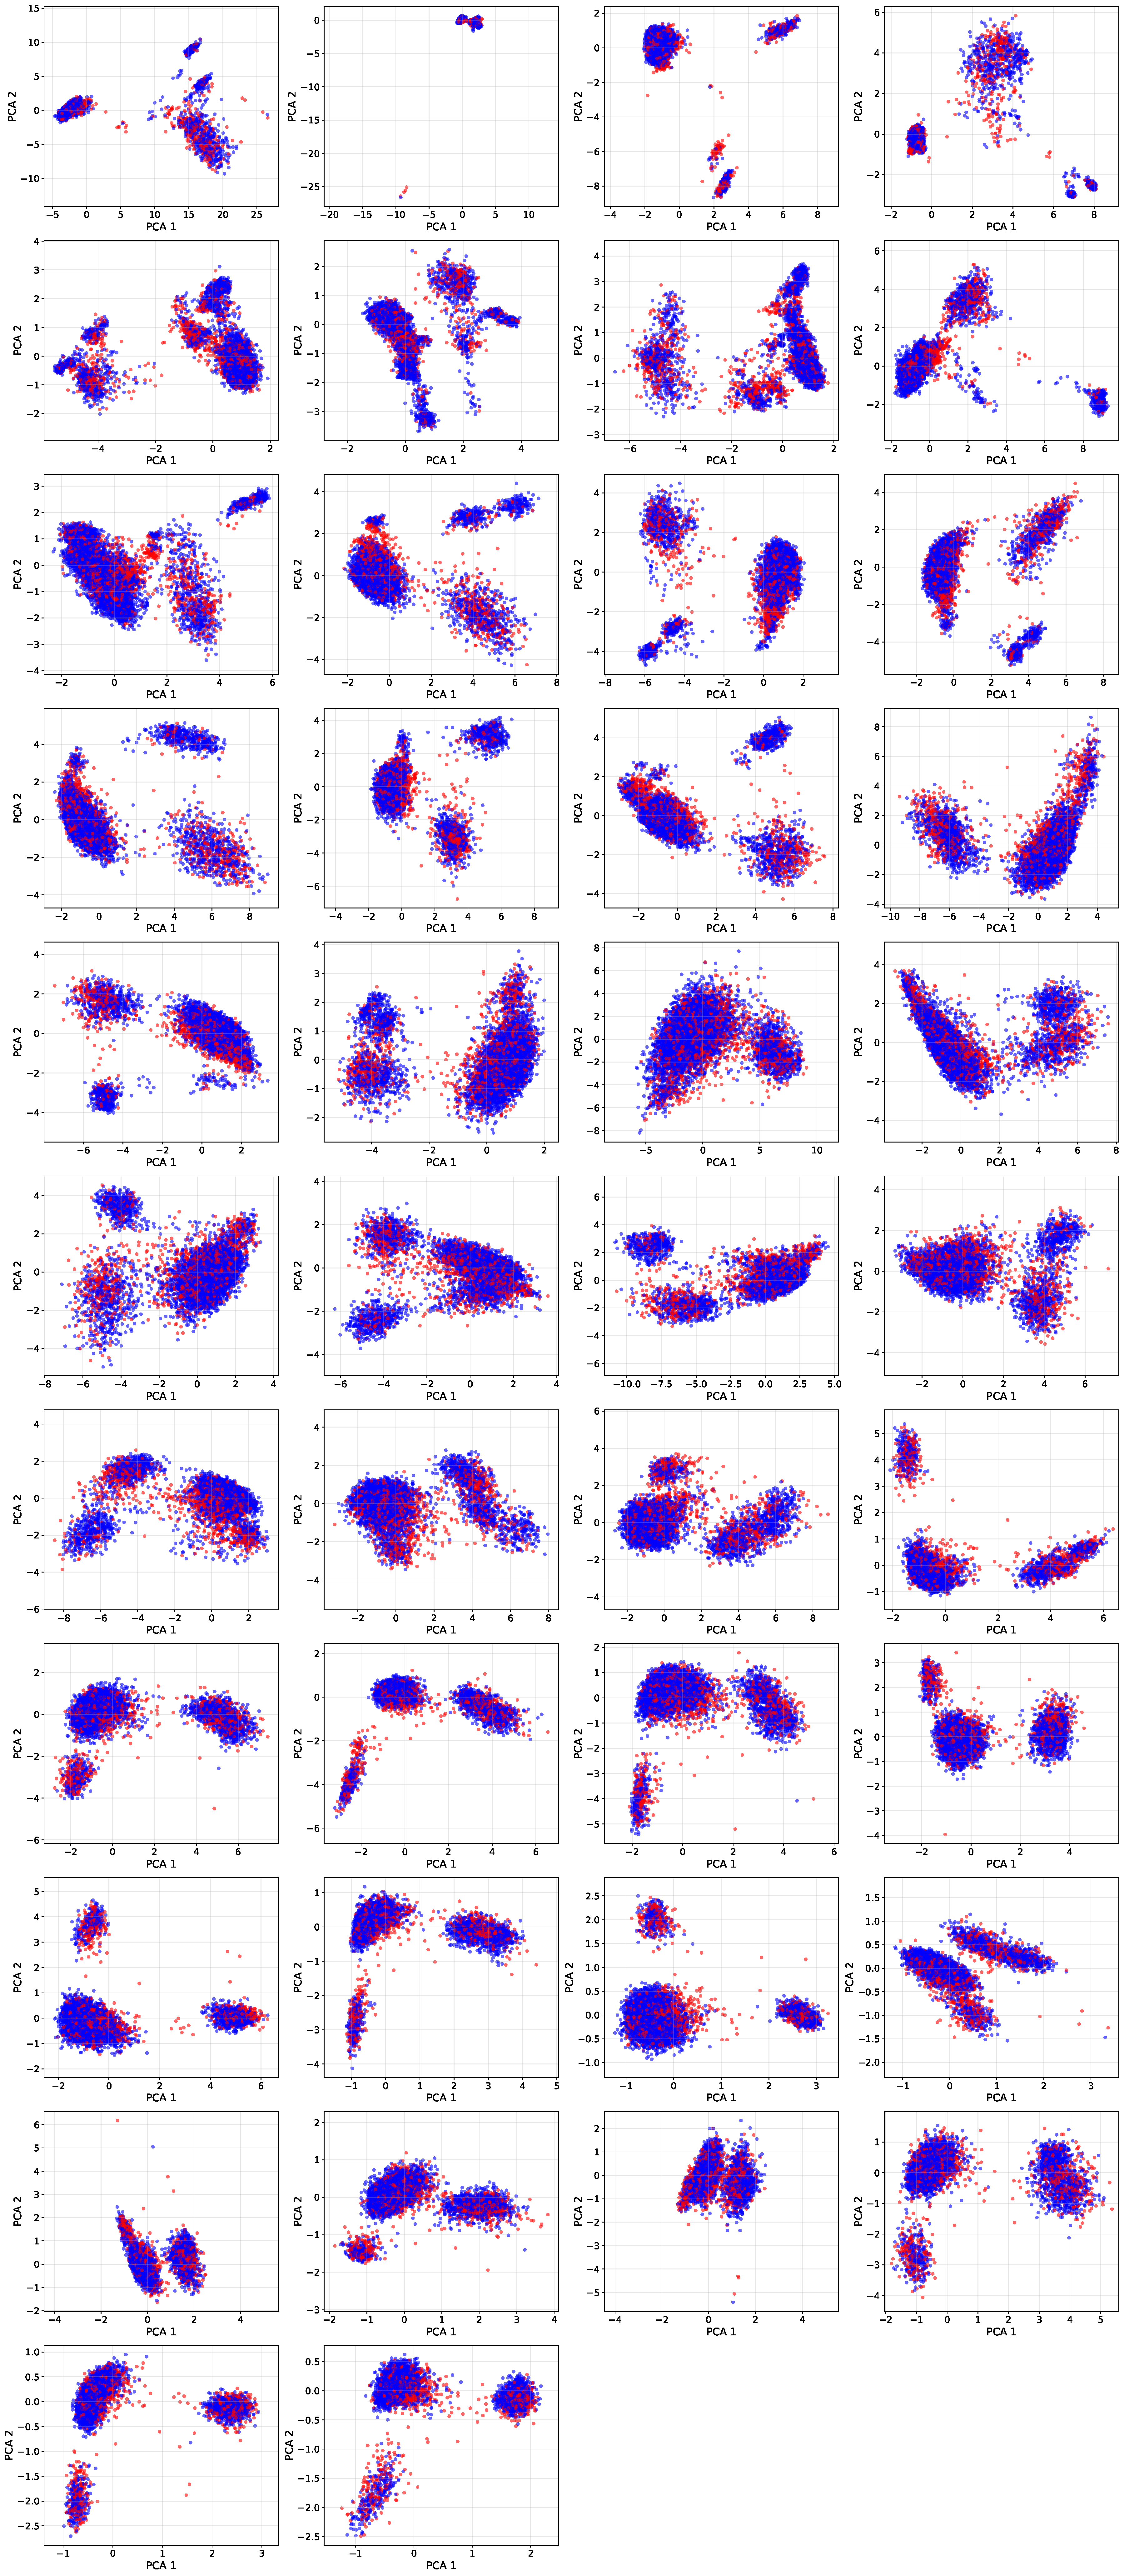
\includegraphics[width=\textwidth, height=1\textheight, keepaspectratio]{images/PCA_Plots/gemma-2-9b-it_halu_eval_attn_activations_PCA_CLEAN.pdf}
    \label{fig:gemma-pca-attn-he-full}
    \caption{PCA delle attivazioni Attention del layer di Gemma-2-9B-IT per Halu Eval}
\end{figure}



\begin{figure}[H]
    \centering
    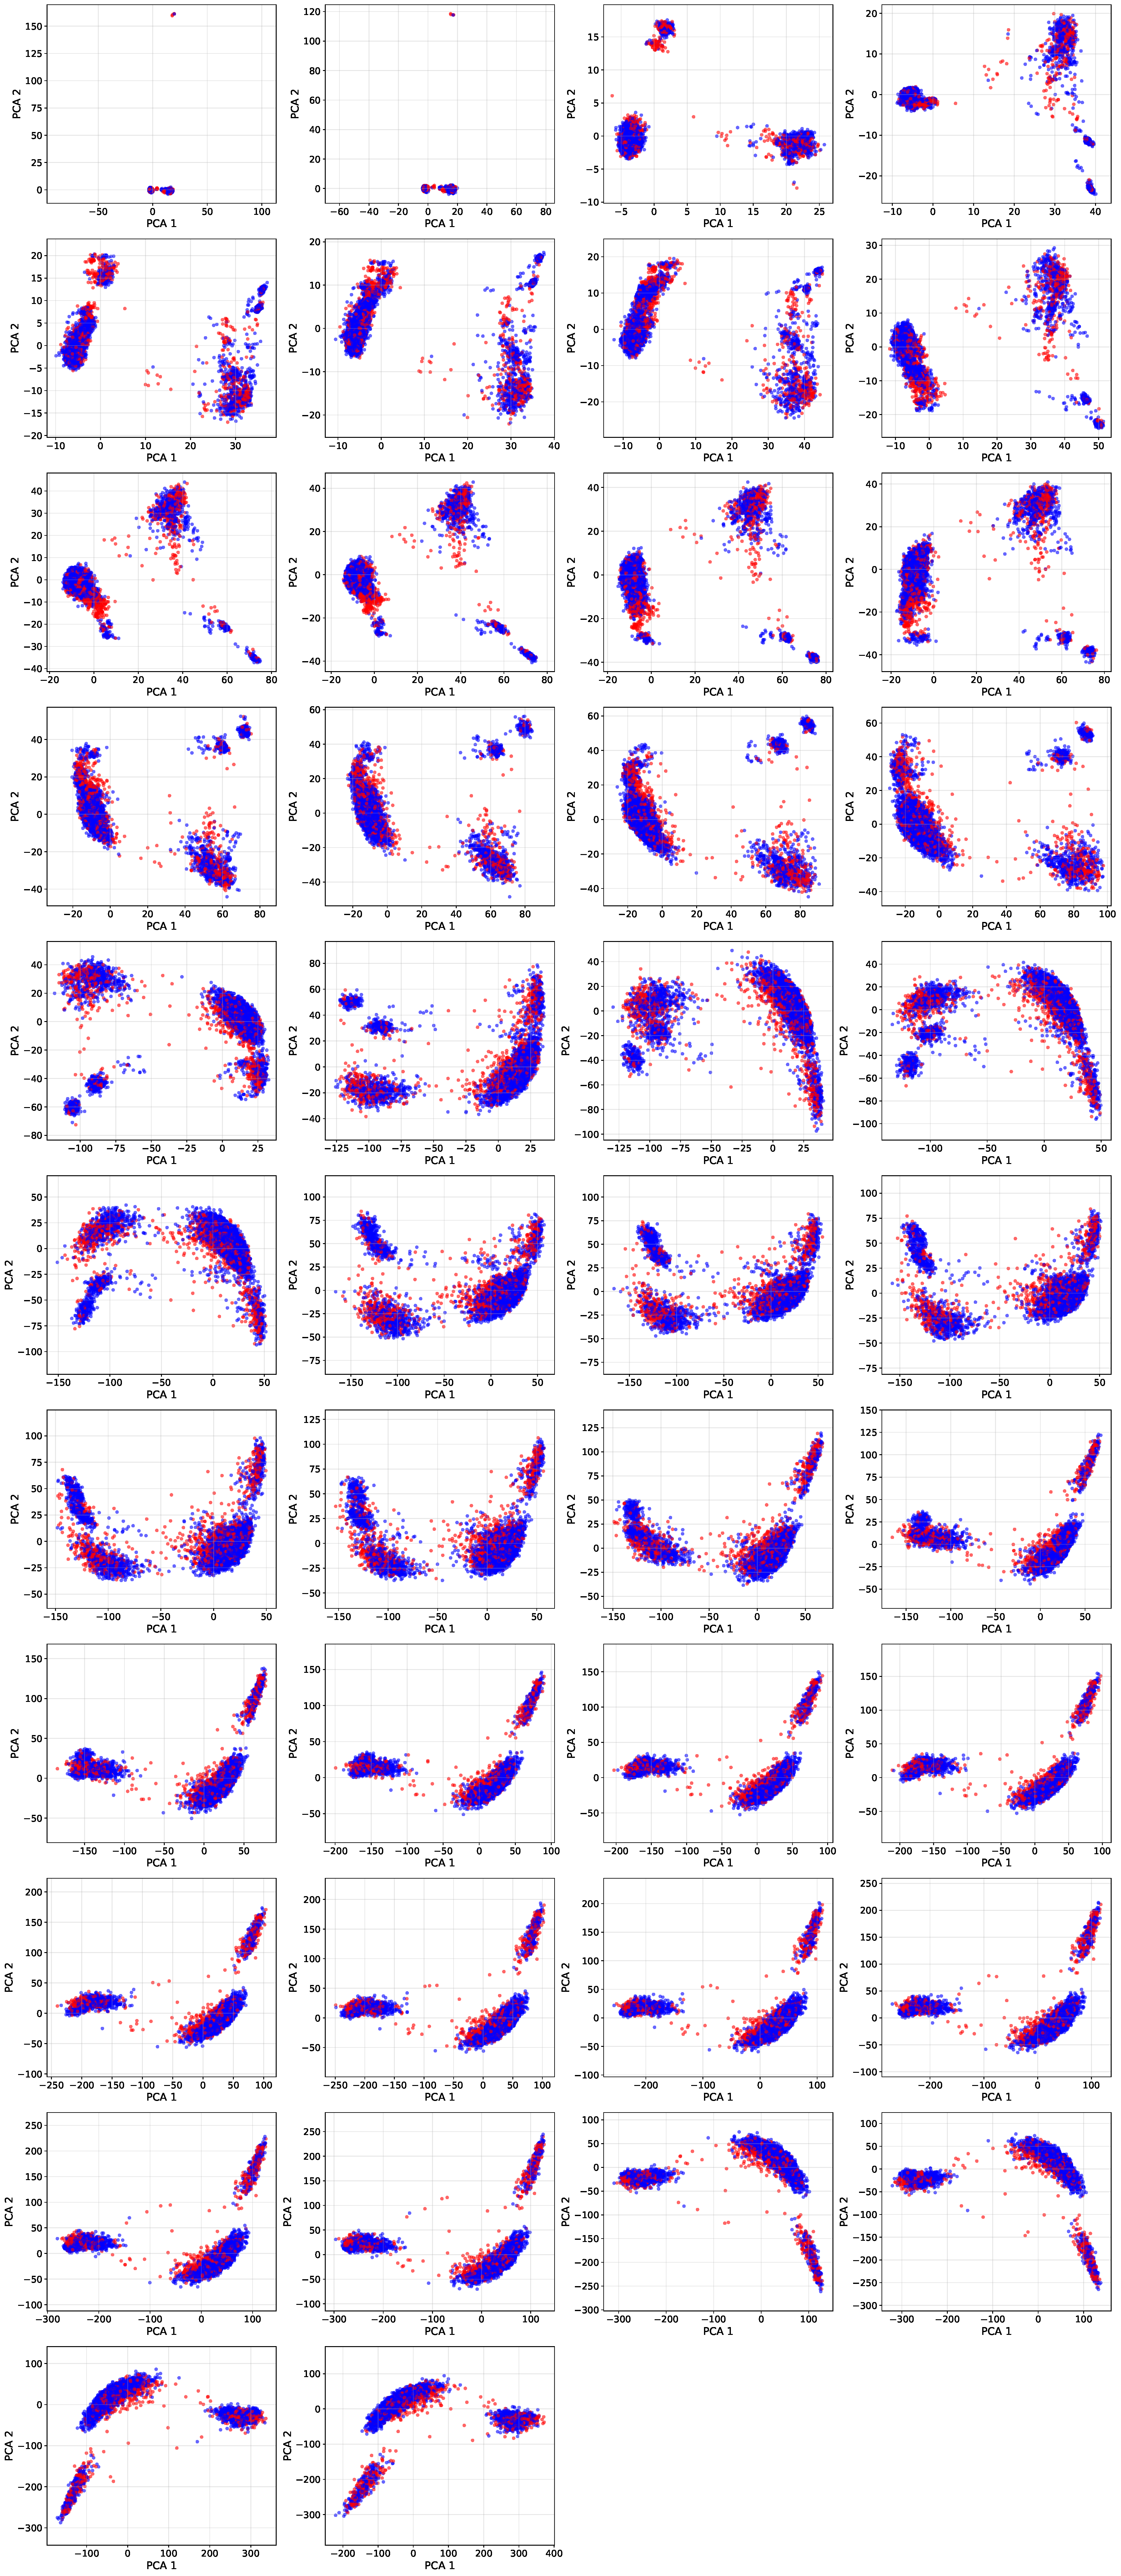
\includegraphics[width=\textwidth, height=1\textheight, keepaspectratio]{images/PCA_Plots/gemma-2-9b-it_halu_eval_hidden_activations_PCA_CLEAN.pdf}
    \label{fig:gemma-pca-hidden-he-full}
    \caption{PCA delle attivazioni Hidden del layer di Gemma-2-9B-IT per Halu Eval}

\end{figure}

\begin{figure}[H]
    \centering
    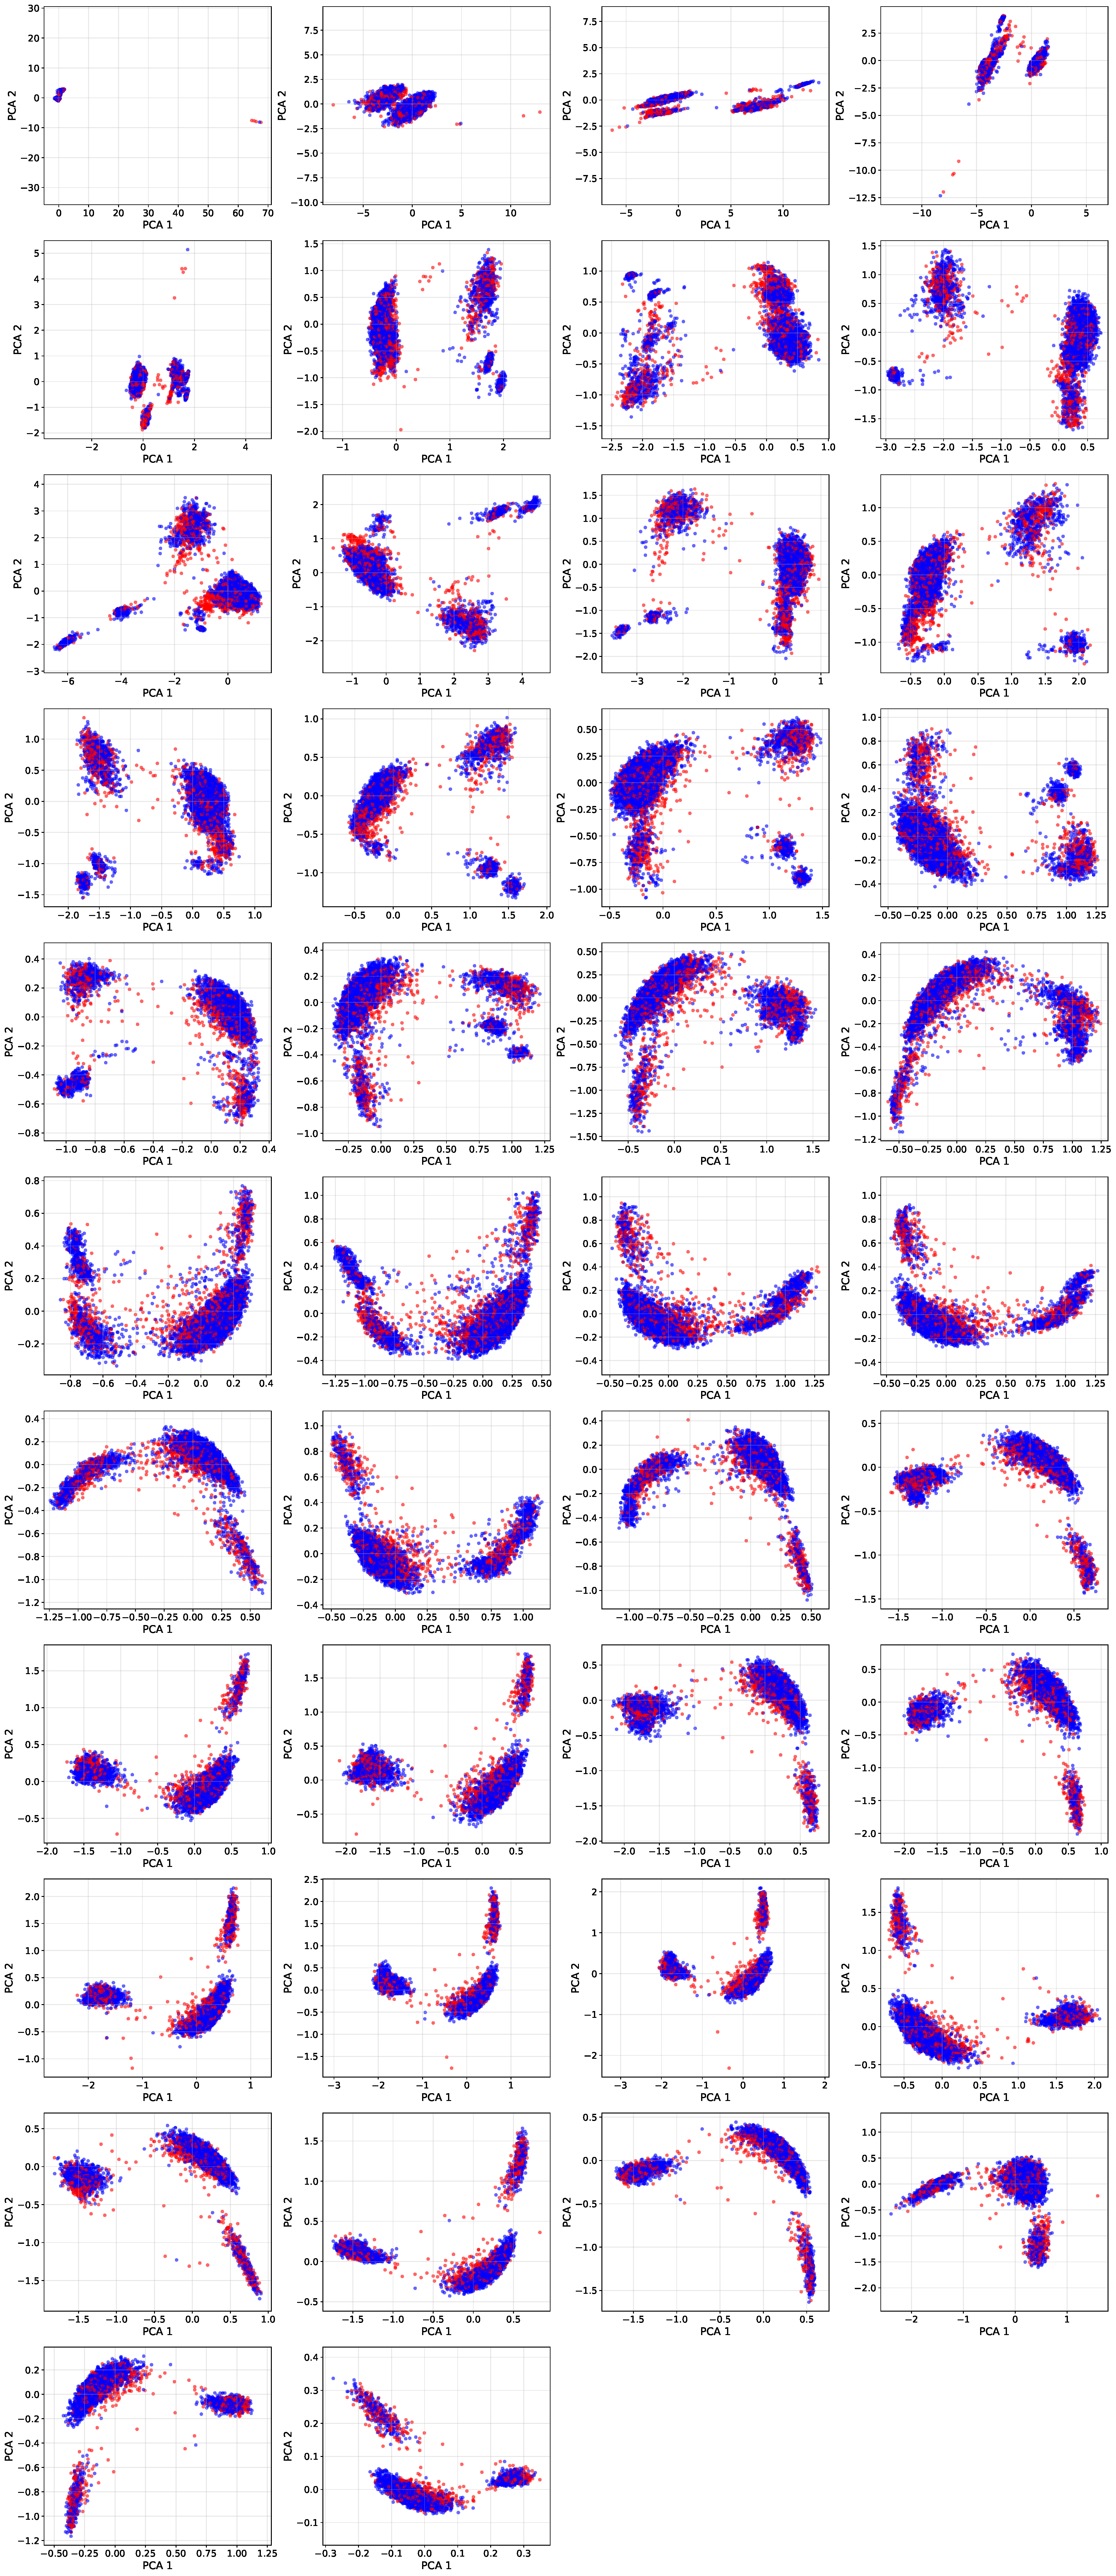
\includegraphics[width=\textwidth, height=1\textheight, keepaspectratio]{images/PCA_Plots/gemma-2-9b-it_halu_eval_mlp_activations_PCA_CLEAN.pdf}
    \label{fig:gemma-pca-mlp-he-full}
    \caption{PCA delle attivazioni MLP del layer di Gemma-2-9B-IT per Halu Eval}
\end{figure}

\begin{figure}[H]
    \centering
    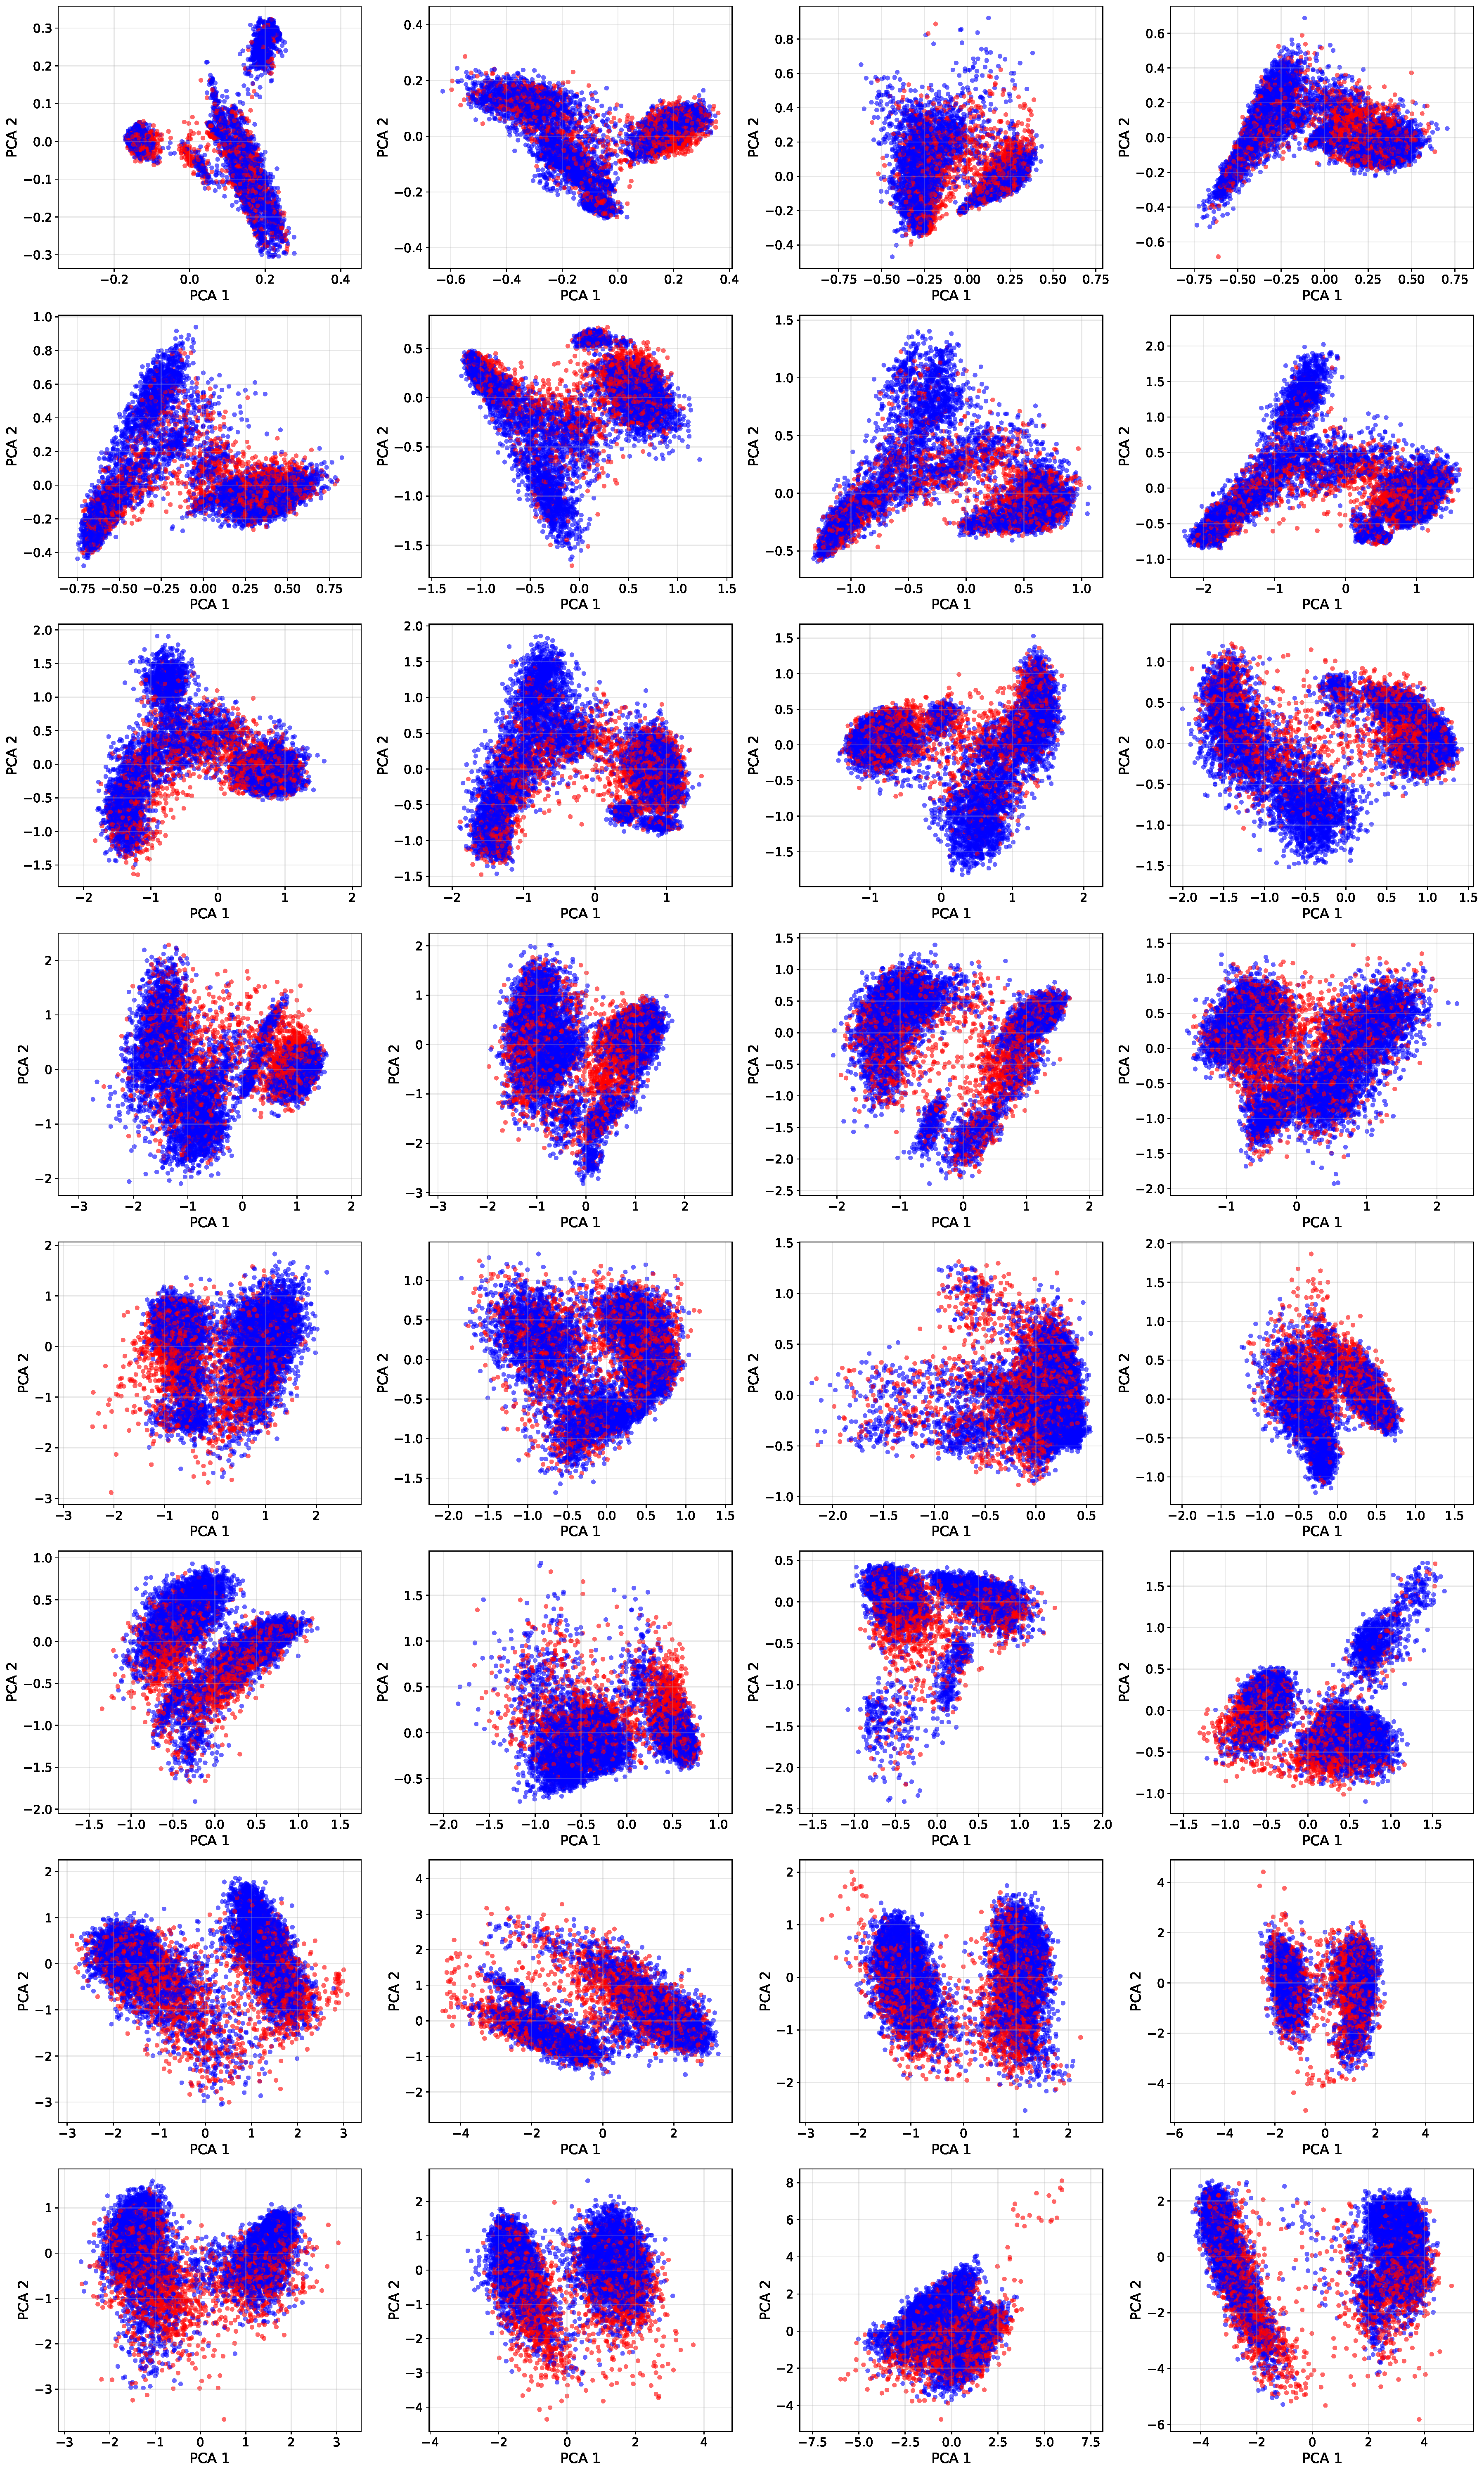
\includegraphics[width=\textwidth, height=1\textheight, keepaspectratio]{images/PCA_Plots/Llama-3.1-8B-Instruct_halu_eval_attn_activations_PCA_CLEAN.pdf}
    \label{fig:llama-pca-attn-he-full}
    \caption{PCA delle attivazioni Attention del layer di Llama-3.1-8B-Instruct per Halu Eval}
\end{figure}

\begin{figure}[H]
    \centering
    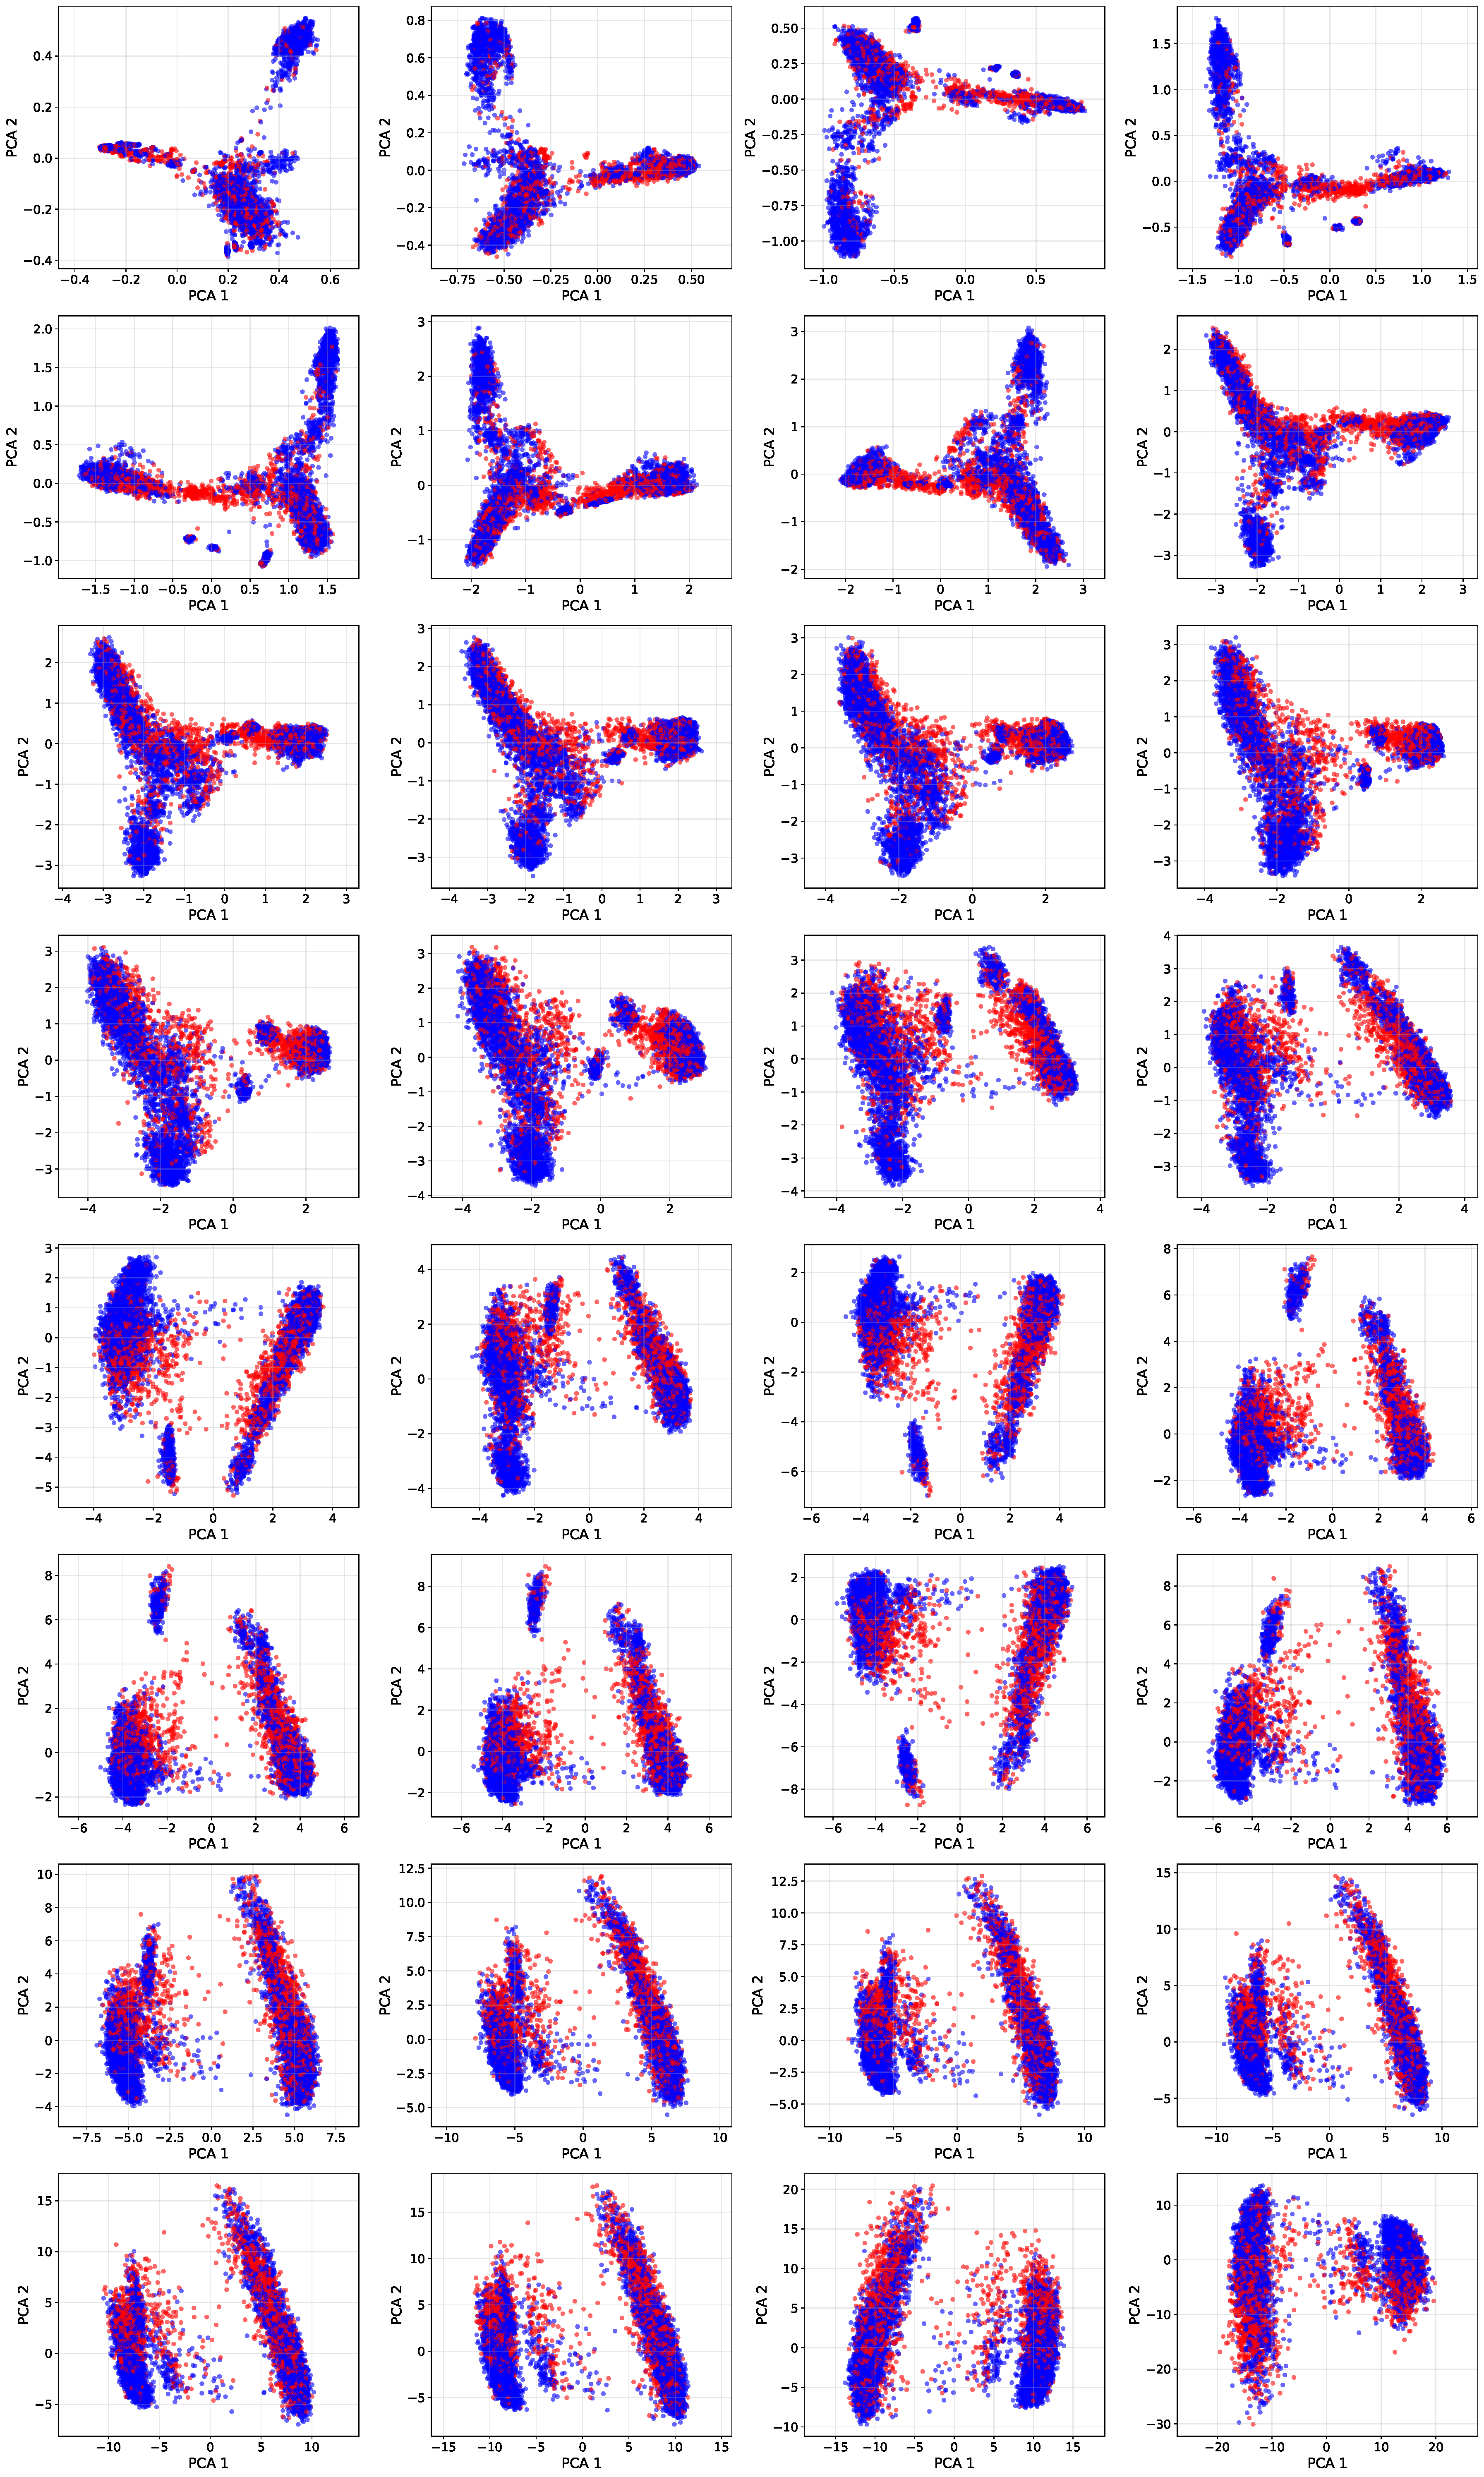
\includegraphics[width=\textwidth, height=1\textheight, keepaspectratio]{images/PCA_Plots/Llama-3.1-8B-Instruct_halu_eval_hidden_activations_PCA_CLEAN.pdf}
    \label{fig:llama-pca-hidden-he-full}
    \caption{PCA delle attivazioni Hidden del layer di Llama-3.1-8B-Instruct per Halu Eval}
\end{figure}

\begin{figure}[H]
    \centering
    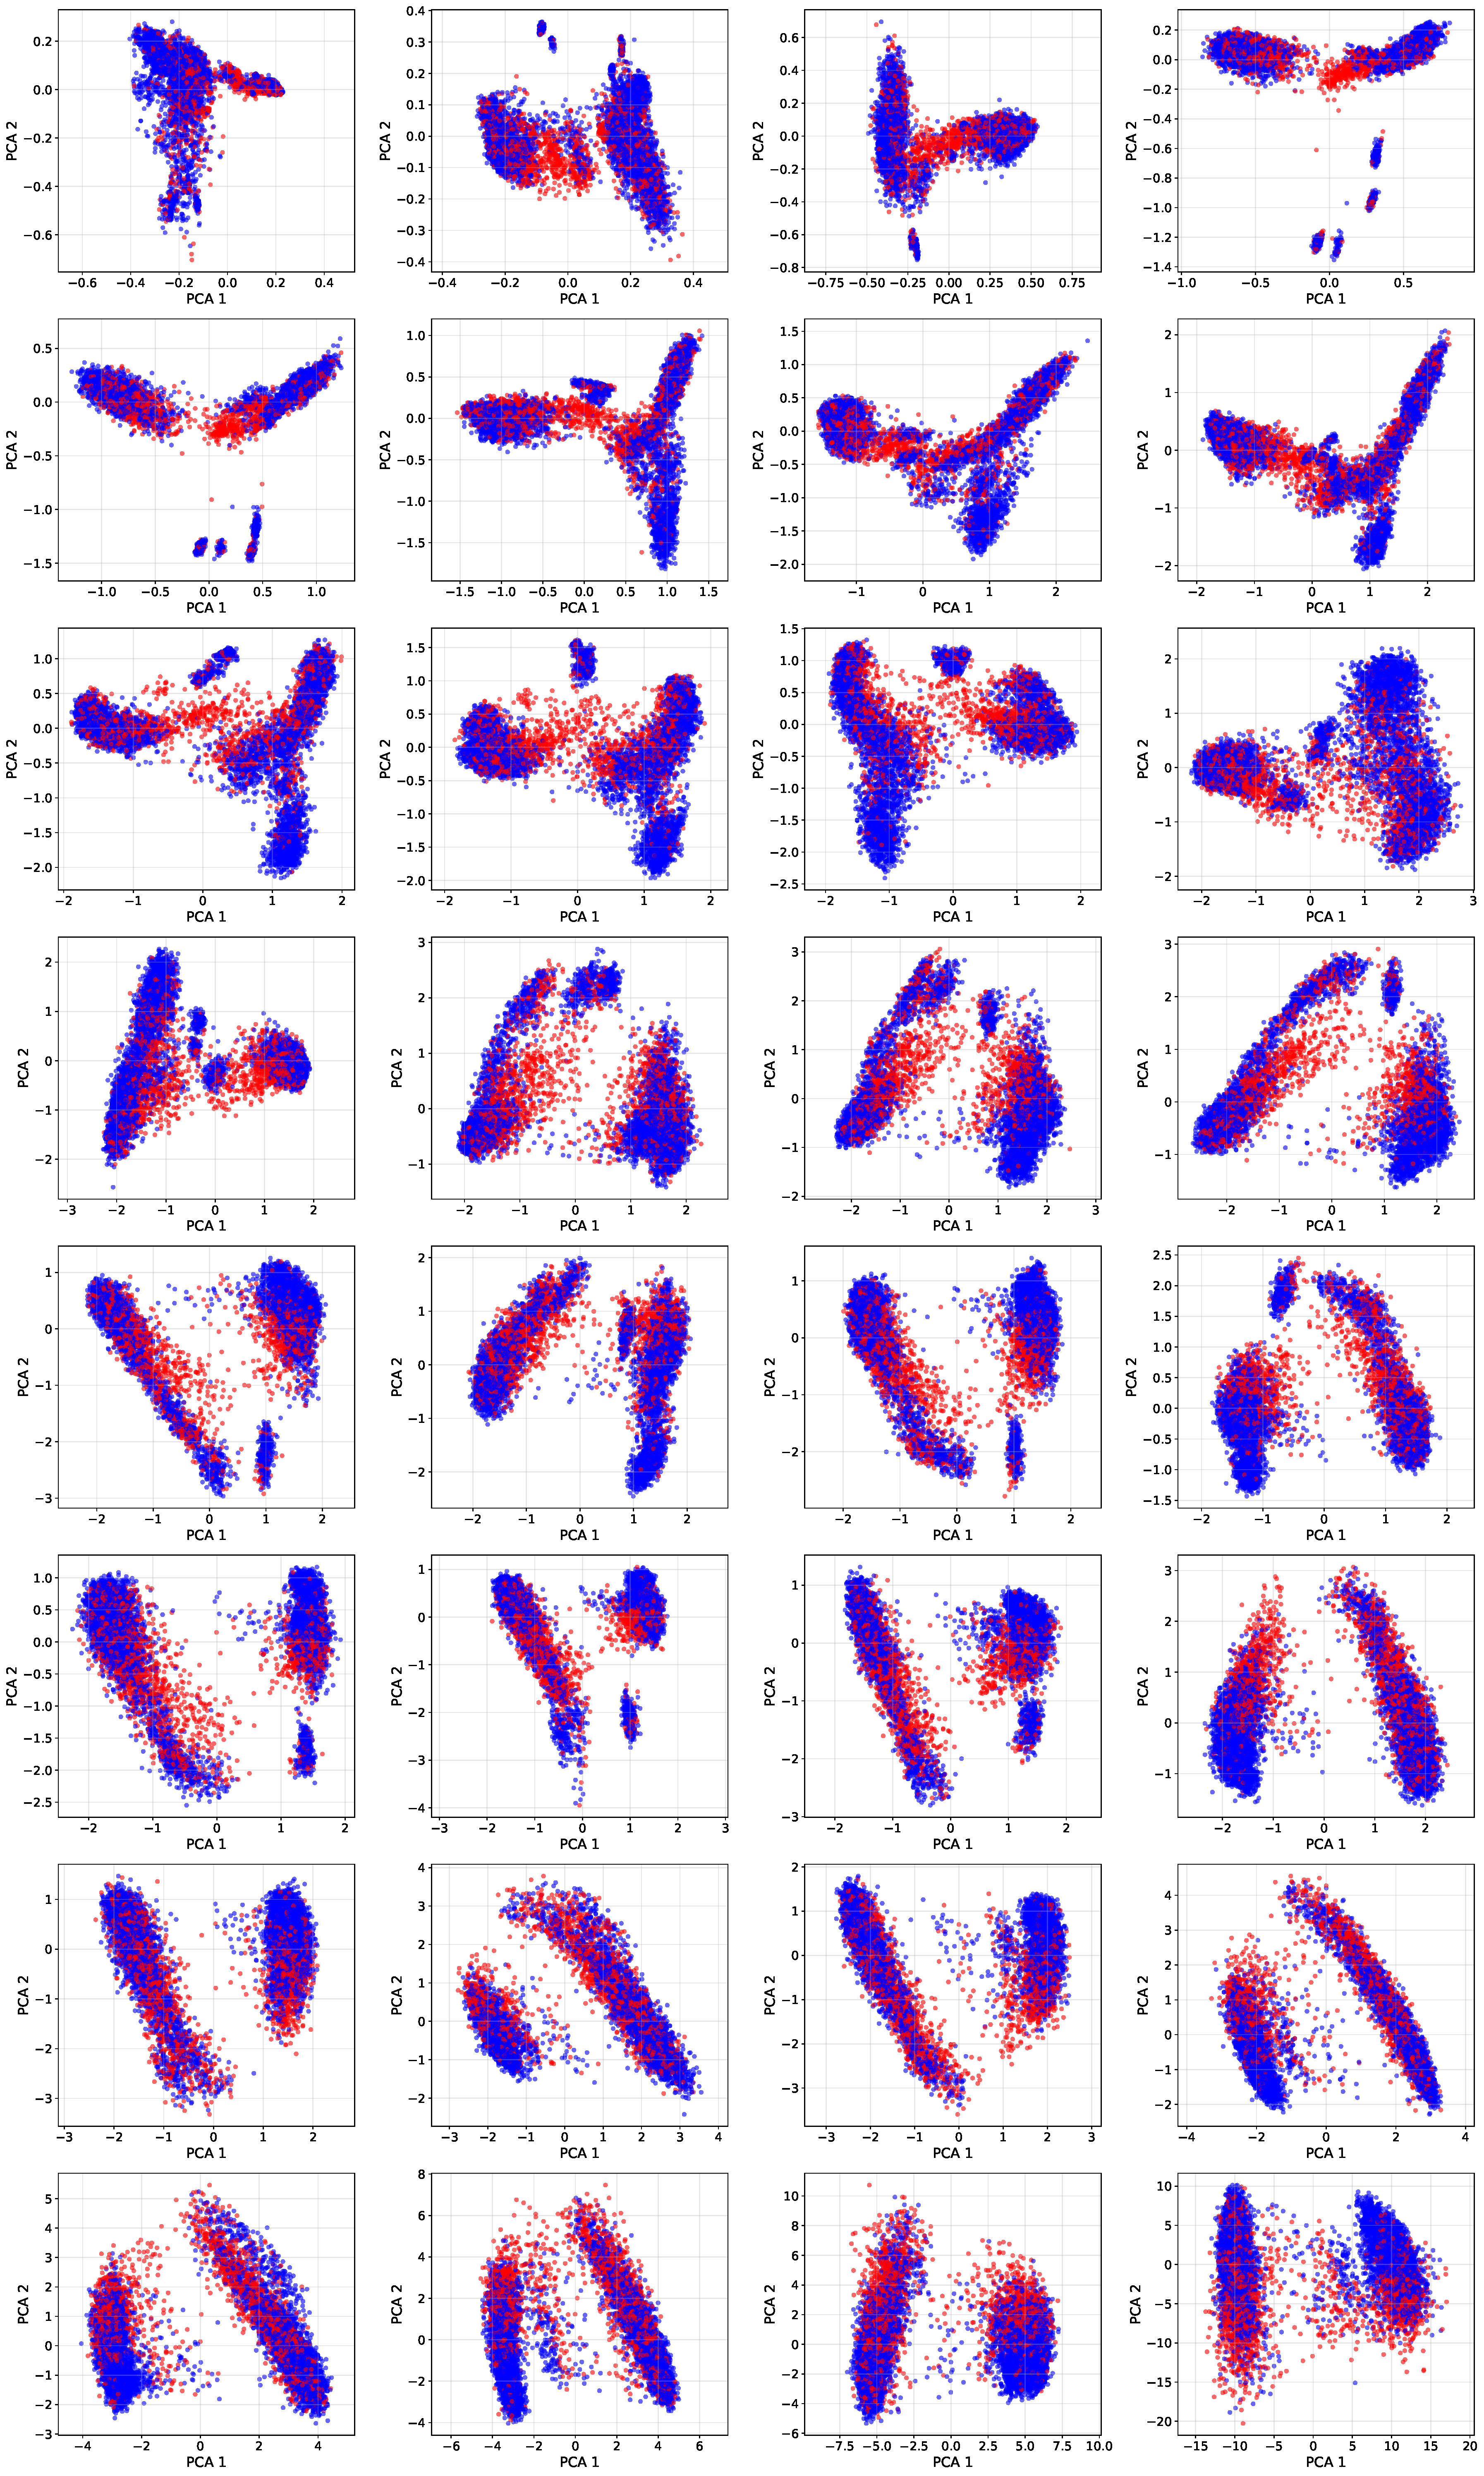
\includegraphics[width=\textwidth, height=1\textheight, keepaspectratio]{images/PCA_Plots/Llama-3.1-8B-Instruct_halu_eval_mlp_activations_PCA_CLEAN.pdf}
    \label{fig:llama-pca-mlp-he-full}
    \caption{PCA delle attivazioni MLP del layer di Llama-3.1-8B-Instruct per Halu Eval}
\end{figure}



